%---------------------------------------------------------------------------%
%-                                                                         -%
%-                          Beamer Template                                -%
%-                                                                         -%
%---------------------------------------------------------------------------%
%- Copyright (C) Huangrui Mo <huangrui.mo@gmail.com> 
%- This is free software: you can redistribute it and/or modify it
%- under the terms of the GNU General Public License as published by
%- the Free Software Foundation, either version 3 of the License, or
%- (at your option) any later version.
%---------------------------------------------------------------------------%
%->> Document class declaration
%---------------------------------------------------------------------------%
\documentclass[compress,table,aspectratio=169,xcolor={usenames,dvipsnames}]{beamer}%
%- Multiple options:
%- [<t|c|b>]% vertical alignment for content, vertically centered is default
%- [<slidestop|slidescentered>]% set frame titles position
%- [compress]% reduce the navigate bars
%- [<red|blue|brown|blackandwhite>]% set navigate bar color
%- [<10pt|11pt|12pt|14pt|17pt>]% set font size for normal text, 11pt is default
%- [table]% support tables
%- [aspectratio=169]% set aspect ratio to 16:9, and frame size to 160mm by 90mm
%- [aspectratio=1610]% set aspect ratio to 16:10, and frame size to 160mm by 100mm
%- [aspectratio=MN]% set aspect ratio to M:N, and frame size to 10*M mm by 10*N mm
%- [xcolor={usenames,dvipsnames}]% issue options to xcolor via a beamer-option
%- Manually adjust aspect ratio: design to 4x3, then expand to target, and live with empty space
%- \documentclass[aspectratio=169]{beamer}
%-     \beamertemplatenavigationsymbolsempty%
%-     \usepackage{pdfpages}%
%- \begin{document}
%-     \setbeamercolor{background canvas}{bg=}%
%-     \includepdf[pages=-]{my-original-presentation.pdf}%
%- \end{document}
%- The default font size may seem small, but the actual size of each frame size is
%- by default just 128mm by 96mm and the viewer application enlarges the frame and font.
%- By specifying a default font size smaller than 11pt one can put more onto each slide,
%- by specifying a larger font size one can fit on less.
%---------------------------------------------------------------------------%
%->> Document settings
%---------------------------------------------------------------------------%
\usepackage[biber,authoryear,tikz,table,xlink]{Style/artrabeamer}% document settings
%- usage: \usepackage[option1,option2,...,optionN]{artrabeamer}
%- Multiple optional arguments:
%- [CJK]% Chinese environment support
%- [bibtex|biber]% set bibliography processor and package
%- [<numbered|authoryear|alpha>]% set citation and reference style
%- <numbered>: textual: Jones [1]; parenthetical: [1]
%- <authoryear>: textual: Jones (1995); parenthetical: (Jones, 1995)
%- <alpha>: textual: not available; parenthetical: [Jon95]
%- [tikz]% provide complex diagrams via tikz package
%- [table]% provide complex tables via ctable package
%- [list]% provide enhanced list environments for algorithm and coding
%- [math]% enable some extra math packages
%- [showonlynote]% show note pages only
%- [showsecnote]% show note pages on second screen
%- [handout]% enable handout output
%- [xlink]% disable link colors
\usepackage{Style/artracom}% user defined commands
%---------------------------------------------------------------------------%
%->> Document inclusion
%---------------------------------------------------------------------------%
%\includeonly{Tex/Sec_Introduction}% selected files compilation
%\includeonlylecture{lecture label}% selected lectures compilation
%---------------------------------------------------------------------------%
%->> Theme settings
%---------------------------------------------------------------------------%
%-
%-> Recommended theme combinations
%-
%- set: [<usetheme>, <useoutertheme>, <useinnertheme>, <usecolortheme>]
%- light: [<CambridgeUS>, <miniframes>, <circle>, <dove|seahorse|beaver|seagull>]
%- light: [<Boadilla|Madrid>, <default>, <circle>, <dove|seahorse|beaver|seagull>]
%- dark: [<Boadilla|Madrid>, <default>, <circle>, <fly|albatross>]
%-
%-> Global themes
%-
\usetheme{CambridgeUS}%
%- Options:
%- [<Boadilla|CambridgeUS|default|...>]
%- It is the complete theme in the sense that they control just about every aspect
%- of a slide's appearance. Think of it as major theme.
%- Theme Matrix (https://www.hartwork.org/beamer-theme-matrix/) contains the
%- various theme and color combinations included with beamer.
%-
%-> Outer themes
%-
%\useoutertheme{}%
%- Options:
%- [<default|infolines|miniframes|smoothbars|sidebar|split|shadow|tree|smoothtree>]
%- An outer theme dictates (roughly) the overall layout of frames. It specifies where
%- any navigational elements should go (like a mini table of contents or navigational
%- mini frames) and what they should look like. Typically, an outer theme specifies
%- how the following elements are rendered:
%- - The headline and footline.
%- - The sidebars.
%- - The logo.
%- - The frame title.
%- The Beamer User Guide explains each theme with examples.
%-
%- *** Miniframes
\useoutertheme[%
    %footline=empty,% suppressed the footline (default).
    %footline=authorinstitute,% shows the author's name and the institute in the footline.
    %footline=authortitle,% shows the author's name and the title in the footline.
    %footline=institutetitle,% shows the institute and the title in the footline.
    %footline=authorinstitutetitle,% shows all three in the footline.
    subsection=false,% shows or suppresses line showing the subsection in the headline.
]{miniframes}%
%-
%- *** Sidebar
%\useoutertheme[%
%    %left,% sidebar links.
%    %right,% sidebar rechts.
%    %hideallsubsections,% suppresses all subsections.
%    %hideothersubsections,% suppresses all subsections except the current one.
%]{sidebar}%
%-
%-> Inner themes
%-
\useinnertheme{circles}%
%- Options:
%- [<default|circles|rectangles|rounded|inmargin>]
%- An inner theme installs templates that dictate how the following elements are typeset:
%- - Title and part pages.
%- - Itemize environments.
%- - Enumerate environments.
%- - Description environments.
%- - Block environments.
%- - Theorem and proof environments.
%- - Figures and tables.
%- - Footnotes.
%- - Bibliography entries.
%-
%-> Color themes
%-
\usecolortheme{dove}%
%- Options:
%- [<dove|seahorse|beaver|seagull|fly|albatross|...>]
%- Control the colors of title, frame title, itemization bullets,
%- and many other elements of a slide show.
%- More detailed configure:\setbeamercolor{beamer_element}{color} for
%- of Beamer elements, e.g.color setup
%\setbeamercolor{title}{fg=red!80!black,bg=red!20!white}
%\setbeamercolor{frametitle}{fg=blue,bg=yellow}
%---------------------------------------------------------------------------%
%->> Configuration
%---------------------------------------------------------------------------%
%-
%-> Set templates
%-
%- As a user of the beamer class you typically do not 'use' or 'invoke'
%- templates yourself, directly. For example, the frame title template
%- is automatically invoked by beamer somewhere deep inside the frame
%- typesetting process. The same is true of most other templates.
%- However, if, for whatever reason, you wish to invoke a template
%- yourself, you can use the following command.
%-\setbeamertemplate{some beamer element}{your definition for this template}
%-
%- *** Headline and footline
%\setbeamertemplate{headline}[infolines theme]
%\setbeamertemplate{footline}[page number]
%- Options: {},[default],[infolines theme],[miniframes theme],[frame number],
%-          [page number],[text line]{ text },...
%- Example for redefine the footline:
%-
%- First define some "beamer color" entries:
%\setbeamercolor{myentry1}{fg=black,bg=red!20}
%\setbeamercolor{myentry2}{fg=black,bg=red!30}
%\setbeamercolor{myentry3}{fg=black,bg=red!40}
%- Syntax for \begin{beamercolorbox}[options]{beamer color} ... \end{beamercolorbox}.
%- footline:
%\setbeamertemplate{footline}{
%  \leavevmode%
%  \hbox{%
%  \begin{beamercolorbox}[wd=.333333\paperwidth,ht=2.25ex,dp=1ex,center]{myentry1}%
%-    \usebeamerfont{author in head/foot}\insertshortauthor
%  \end{beamercolorbox}%
%  \begin{beamercolorbox}[wd=.333333\paperwidth,ht=2.25ex,dp=1ex,center]{myentry2}%
%-    \usebeamerfont{title in head/foot}\insertshorttitle
%  \end{beamercolorbox}%
%  \begin{beamercolorbox}[wd=.333333\paperwidth,ht=2.25ex,dp=1ex,right]{myentry3}%
%-    \usebeamerfont{date in head/foot}\insertshortdate{}\hspace*{2em}
%    \insertframenumber{} / \inserttotalframenumber\hspace*{2ex}
%  \end{beamercolorbox}}%
%  \vskip0pt%
%}
%- headline:
%\setbeamertemplate{headline}{
%  \leavevmode%
%  \hbox{%
%  \begin{beamercolorbox}[wd=.5\paperwidth,ht=2.65ex,dp=1.5ex,right]{myentry1}%
%    \usebeamerfont{section in head/foot}\insertsectionhead\hspace*{2ex}
%  \end{beamercolorbox}%
%  \begin{beamercolorbox}[wd=.5\paperwidth,ht=2.65ex,dp=1.5ex,left]{myentry3}%
%    \usebeamerfont{subsection in head/foot}\hspace*{2ex}\insertsubsectionhead
%  \end{beamercolorbox}}%
%  \vskip0pt%
%}
%- Change the footer/footline of a single frame in Beamer: use {} to confine effect domain.
%- The \leavevmode ensures that the vertical mode is ended and horizontal mode is entered. 
%- In vertical mode, TeX stacks horizontal boxes vertically, whereas in horizontal mode, 
%- they are taken as part of the text line. Use \leavevmode for all macros which could be 
%- used at the begin of the paragraph and add horizontal boxes by themselves.
%-
%- *** Outline setting
%\AtBeginPart% [<Lecture|Part|Section>]% insert content at the beginning of each element
%{%
%    \frame[plain]{\partpage}% [<partpage|sectionpage>][<\insertlecture|\insertpart|\insertsection>]
%    \begin{frame}[plain]%
%        \frametitle{Outline}%
%        {%
%            \tableofcontents[sectionstyle=show/shaded,subsectionstyle=show/show/shaded]%
%        }%
%    \end{frame}%
%}
%- - sectionstyle=<style for current section>/<style for other sections>
%- - subsectionstyle=<style for current subsection>/<style for other
%-   subsections in current section>/<style for subsections in other sections>
%- - Allowed <styles> are show, shaded, and hide.
%- Other options:
%- - currentsection, equal to: sectionstyle=show/shaded,subsectionstyle=show/show/shaded
%- - currentsubsection, equal to: subsectionstyle=show/shaded.
%- - firstsection=<section number> specifies which section should be numbered as section "1."
%-   This is useful if you have a first section (like an overview section) that should not
%-   receive a number.
%- - hideallsubsections, equal to: subsectionstyle=hide.
%- - pausesections, causes a \pause command to be issued before each section.
%-   This is useful if you wish to show the table of contents in an incremental way.
%-
%- *** Navigation symbols
\setbeamertemplate{navigation symbols}{}% suppresses all navigation symbols.
%\setbeamertemplate{navigation symbols}[only frame symbol]% only for navigating frames.
%-
%- *** Frame title
%\setbeamertemplate{frametitle}[default][left]% left, center, right
%-
%- *** Background
%\setbeamertemplate{background}[grid][step=\grid,color=blue]
%\setbeamertemplate{background canvas}[default]
%\setbeamertemplate{background canvas}[vertical shading][bottom=red!20,top=yellow!30]
%\setbeamertemplate{background canvas}{\includegraphics[width=\paperwidth,height=\paperheight]{alps.jpg}}
%\tikzart[t=c]{cover_front_thu_cce}
%\tikzart[t=c]{cover_composite_tonemapped}[trim=0mm 100mm 0mm 0mm,clip]
%- The aspect ratio of a Beamer slide is 4:3 therefore it's best
%- if your background image has the same aspect ratio. Otherwise
%- your image will be distorted when it's stretched to cover the
%- slide from edge to edge.
%- To limit the background setting to a single slide, enclose the
% \setbeamertemplate{background canvas}{...} command in braces,
%- as in:
%-
%{% brace to limit the scope of \setbeamertemplate
%\setbeamertemplate{navigation symbols}{}% optionally hide navigation buttons
%\setbeamertemplate{background canvas}{\includegraphics
%	[width=\paperwidth,height=\paperheight]{alps.jpg}}
%\begin{frame}[plain]
%...
%\end{frame}
%}% closing brace
%-
%- *** Margin sizes
%\setbeamersize{text margin left=2em,text margin right=2em}
%-
%- *** Itemizations, enumerations, and descriptions
%\setbeamertemplate{itemize items}[triangle]
%- Options: [<circle|triangle|square|ball>].
%\setbeamertemplate{enumerate items}[default]
%- Options:
%- [default]% numbered
%- [sections numbered]% section numbered, subsections are not numbered.
%- [subsections numbered]% subsections are numbered, but not the sections.
%- [circle]% numbered circles before section, not subsection.
%- [square]% numbered squares before section. unnumbered squares before subsections.
%- [ball]% similar to square, but use balls.
%- [ball unnumbered]% similar to ball, except that no numbering is used.
%-
%- *** Block environments
%\setbeamertemplate{blocks}[rounded][shadow=true]
%- Types:
%- "theorem", "corollary", "definition" in structure color frame.
%- "examples" in green color frame.
%- "block" in structure color frame with your own title.
%- "alertblock" in alert color frame with your own title.
%-
%- *** Theorem environments
%\setbeamertemplate{theorems}[normal font]
%- Options: [<default|normal font|numbered|ams style>].
%-
%- *** Figures and tables
%\setbeamertemplate{caption}[default]
%- Options:
%- [default]% typesets the caption name (a word like 'Figure' or 'Abbildung' or 'Table')
%- [numbered]% adds the figure or table number to the caption.
%- [caption name own line].
%-
%- *** Adding sections and subsections
%\setbeamertemplate{sections/subsections in toc}[square]
%- Options: [<default|sections numbered|subsections numbered>]
%-          [<circle|square|ball|ball unnumbered>]
%-
%- *** Bibliography
\setbeamertemplate{bibliography item}{}% remove the icon
%-
%-> Fonts
%-
%- Set fonts used for different elements of a slide via Beamer's Font Management.
%- Rules:
%\setbeamerfont{some beamer element}{size=\large}
%- Add * to the command to first completely "reset" the font attributes.
%- Options:
%- parent=structure,size=\large,series=\bfseries,shape=\itshape,family=\sffamily.
%- Explains: there are three familis of font
%- family: \rmfamily(serif) or \sffamily(sans serif), or \ttfamily(monospace).
%- Each family has its own font characteristics, i.e., font properties.
%- shapes: \itshape, \slshape, \scshape, or \upshape.
%- series(light, bold,...): \bfseries, \mdseries.
%-
%- *** Structure font
%\setbeamerfont{structure}{}
%\setbeamerfont{tiny structure}{size=\tiny}
%-
%- *** Normal font
%\setbeamerfont{normal text}{parent=structure,size=\small}% ignored currently
%\setbeamerfont{alerted text}{}
%\setbeamerfont{example text}{}
%-
%- *** Projected text font
%\setbeamerfont{projected text}{parent={tiny structure}}
%-
%- *** Titlepage font
%\setbeamerfont{title}{parent=structure, size=\large}% shape=\itshape,family=\rmfamily
%\setbeamerfont{title in head/foot}{parent=title, size=\tiny}
%\setbeamerfont{subtitle}{parent=title, size=\normalsize}
%\setbeamerfont{author}{parent=title, size=\normalsize}
%\setbeamerfont{author in head/foot}{parent=title, size=\tiny}
\setbeamerfont{institute}{parent=structure, size=\normalsize, series=\mdseries}
%\setbeamerfont{institute in head/foot}{parent=title, size=\tiny}
%\setbeamerfont{date}{parent=institute}
%\setbeamerfont{date in head/foot}{parent=title, size=\tiny}
%-
%- *** Frame title font
\setbeamerfont{frametitle}{parent=structure,size=\large}
%\setbeamerfont{framesubtitle}{parent=frametitle,size=\footnotesize}
%-
%- *** Part fonts
%\setbeamerfont{part name}{size=\Large}
%\setbeamerfont{part title}{parent=title}
%-
%- *** Headline and footline font
%\setbeamerfont{headline}{parent={tiny structure}}
%\setbeamerfont{footline}{parent={tiny structure}}
%-
%- *** Caption font
%\setbeamerfont{caption}{size=\small}
%\setbeamerfont{caption name}{size=\small}
%-
%- *** Button font
%\setbeamerfont{button}{size=\tiny}
%-
%-> Transparent effect
%-
%\setbeamercovered{invisible}
%- Options:
%- [invisible]% is the default and causes covered text to disappear.
%- [transparent]% creates shaded instead of hidden overlays.
%- [dynamic]% makes all covered text quite transparent, but in a dynamic way.
%- [highly dynamic]% has the same effect as dynamic, but the effect is stronger.
%\beamerdefaultoverlayspecification{<+->}% uncover everything in a step-wise fashion
%---------------------------------------------------------------------------%
%->> Document content
%---------------------------------------------------------------------------%
%-
%-> Titlepage information
%-
%---------------------------------------------------------------------------%
%->> Document inclusion
%---------------------------------------------------------------------------%
%\includeonly{Tex/Sec_Introduction,Tex/Sec_Method,Tex/Sec_Result,Tex/Sec_Conclusion}% selected files compilation
%\includeonlylecture{lec_present_intro,lec_present_method,lec_present_result,lec_present_conclude}% selected lectures compilation
%\includeonlyframes{fra_current}% selected frames compilation
%---------------------------------------------------------------------------%
%->> Titlepage information
%---------------------------------------------------------------------------%
\title[]% optional, abbreviated title
{"Honey, I shrunk the parameters": A Comparison of Lasso, Ridge, and Elastic Net Methods}
\subtitle{}


\author[]% optional, abbreviated authors
{Carolina Alvarez, Edoardo Falchi, and Emily Anne Schwab}

\institute[]% optional, abbreviated name
{
  %\inst{*}%
  %\enorcn{Mechanical and Mechatronics Engineering, University of Waterloo}{\small 加拿大滑铁卢大学}
  %\and
  %\inst{\dag}%
  %\enorcn{Center for Combustion Energy, Tsinghua University}{\small 清华大学燃烧能源中心}
  %\and
  %\inst{+}%
  {Research Module in Econometrics and Statistics}
}

\date{\today}

\subject{Report by Huangrui Mo}% inserted into the PDF information catalog

%\logo{\tikzart[t=p,x=8,y=-6,w=4]{logo_uw}}% on each slide 
\titlegraphic{\tikzart[t=p,x=0,y=-4,w=4]{bonn-logo}}% only on title page
% can also use any field given by \author, \title, \date, \institute, or \tikz to place image in the title page
%\addtobeamertemplate{headline}{}{% on each slide with headline
%    \tikzart[t=p,x=8,y=7,w=4]{logo_uw}
%}
%---------------------------------------------------------------------------%
%
\begin{document}
%-
%-> Frontmatter
%-
%---------------------------------------------------------------------------%
%->> Frontmatter
%---------------------------------------------------------------------------%
%---------------------------------------------------------------------------%
%->> Create titlepage
%---------------------------------------------------------------------------%
%- create the title page, \frame[plain]{\titlepage} for a titlepage filling the whole frame.
{% these braces make the change local to the single frame.
    \setbeamertemplate{headline}{%
        \begin{beamercolorbox}[wd=\paperwidth,ht=2.5ex,dp=1.5ex,right]{section in head/foot}%
        \end{beamercolorbox}%
    }
    \setbeamertemplate{footline}{%
        \leavevmode%
        \hbox{%
            \begin{beamercolorbox}[wd=.333333\paperwidth,ht=2.25ex,dp=1ex,center]{author in head/foot}%
            \end{beamercolorbox}%
            \begin{beamercolorbox}[wd=.333333\paperwidth,ht=2.25ex,dp=1ex,center]{title in head/foot}%
            \end{beamercolorbox}%
            \begin{beamercolorbox}[wd=.333333\paperwidth,ht=2.25ex,dp=1ex,right]{date in head/foot}%
            \end{beamercolorbox}}%
        \vskip0pt%
    }
    \begin{frame}[plain]
        \titlepage%
        %\tikzart[t=p,x=0,y=-4,w=4]{logo_uw}
        \addtocounter{framenumber}{-1}% modify the counter to exclude a frame from total count
    \end{frame}%
}
%---------------------------------------------------------------------------%
%->> Outline page
%---------------------------------------------------------------------------%
%\section[Outline]{}%
%\begin{frame}[plain]%
%    \frametitle{Outline}%
%    \tableofcontents%[part=partid]% may add the option [pausesections]
%    \addtocounter{framenumber}{-1}% modify the counter to exclude a frame from total count
%\end{frame}%
\AtBeginPart% [<Lecture|Part|Section>]% insert content at the beginning of each element
{%
    \frame[plain]{\partpage}% [<partpage|sectionpage>][<\insertlecture|\insertpart|\insertsection>]
    %\begin{frame}[plain]%
    %    \frametitle{Outline}%
    %    {%
    %        \tableofcontents[sectionstyle=show/show,subsectionstyle=show/show/show]%
    %    }%
    %\end{frame}%
}
%---------------------------------------------------------------------------%
%->> Content centering
%---------------------------------------------------------------------------%
%\centering% automatic horizontal centering of frame content
%---------------------------------------------------------------------------%
%
%-
%-> Mainmatter
%-
%---------------------------------------------------------------------------%
%->> Main content
%------------------------------------------------------
%---------------------------------------------------------------------------%
%->> Table of contents
%---------------------------------------------------------------------------%
%---------------------------------------------------------------------------%
\lecture{Research Presentation}{lec_present_intro}
%---------------------------------------------------------------------------%
\section{Contents}%
%---------------------------------------------------------------------------%
\begin{frame}[fragile]
    \frametitle{Table of Contents}
    \begin{enumerate}
        \item {Introduction}
        \item {Statistical Properties of Regularization Methods}
            \begin{itemize}
                \item {Ridge}
                \item {Lasso}
                \item {Elastic Net}
            \end{itemize}
        \item {Simulation Studies}
            \begin{itemize}
                \item Comparison of Training MSE 
                \item Selecting an Optimal Tuning Parameter
            \end{itemize}
        \item {Data Application}
            \begin{itemize}
                \item Data Set Overview
                \item Coefficient Paths
                \item Model Selection
            \end{itemize}
        \item {Concluding Remarks}
    \end{enumerate}
\end{frame}

%
%--------------------------------------------------------
%->> Introduction
%---------------------------------------------------------------------------%
%---------------------------------------------------------------------------%
\lecture{Research Presentation}{lec_present_intro}
%---------------------------------------------------------------------------%
\section{Introduction}%
%---------------------------------------------------------------------------%
\begin{frame}[fragile]
    \frametitle{Introduction: Drawbacks to OLS}
    \begin{itemize}
        \item Consider the following multivariate linear regression, where $Y=X\beta + \varepsilon$: 
            \begin{itemize}
                \item $Y=(y_1,...,y_n)$ $\in$ ${\rm I\!R^{n}}$ is the response vector
                \item $X$ $\in$ ${\rm I\!R^{n \times p}}$ is the predictor variable matrix
                \item $\varepsilon=¨(\varepsilon_1,...,\varepsilon_n)$ is the error vector
            \end{itemize}
        \item When is OLS a sub-optimal model for prediction? 
            \begin{itemize}
                \item Imperfect multicollinearity
                    \begin{itemize}
                        \item $cov(X_i, X_j)\neq 0$
                        \item $\beta_{OLS}$ still BLUE, but variance and standard errors will increase.
                        \item Leads to lower t-statistics.
                    \end{itemize}
                \item High-dimensionality ($p > n$)
                    \begin{itemize}
                        \item Rank $(X)$ $<$ $p$ such that OLS does not generate a unique solution.
                        \item Variance of estimated coefficients becomes infinitely large.
                    \end{itemize}
            \end{itemize}
    \end{itemize}
\end{frame}
%---------------------------------------------------------------------------%
\begin{frame}[fragile, c]
\frametitle{Regularization Methods}
    \begin{center}
        \textbf{Solution:} Use regularization method(s) to reduce the variance of the model fit in exchange for a marginal increase in the bias.
    \end{center}
\end{frame}
%
%---------------------------------------------------------------------------%
%->> Method
%---------------------------------------------------------------------------%
%---------------------------------------------------------------------------%
\lecture{Research Presentation}{lec_present_method}
%---------------------------------------------------------------------------%
\section{Theory}
%---------------------------------------------------------------------------%
\begin{frame}[fragile]
    \frametitle{Ridge Regression}
    Similar to OLS, ridge minimizes the sum of squared residuals (SSR), but includes an $\ell_2$-norm shrinkage penalty with a tuning parameter ($\lambda$):
    \begin{align}
    \label{eqn:eqn1}
    \underbrace{\sum_{i=1}^{n}\left(y_{i}-\beta_{0}-\sum_{j=1}^{p} \beta_{j} x_{i j}\right)^{2}}_\text{SSR} + \underbrace{\lambda\sum_{j=1}^{p}\beta_{j}^{2}.}_\text{shrinkage penalty}
    \end{align}
    \begin{itemize}
        \item If $\lambda=0$, we are left with the OLS estimates.
        \item As $\lambda$ increases, the estimated ridge coefficients shrink towards zero.
    \end{itemize}
\end{frame}
%---------------------------------------------------------------------------%
\begin{frame}[fragile]
    \begin{figure}[b]
        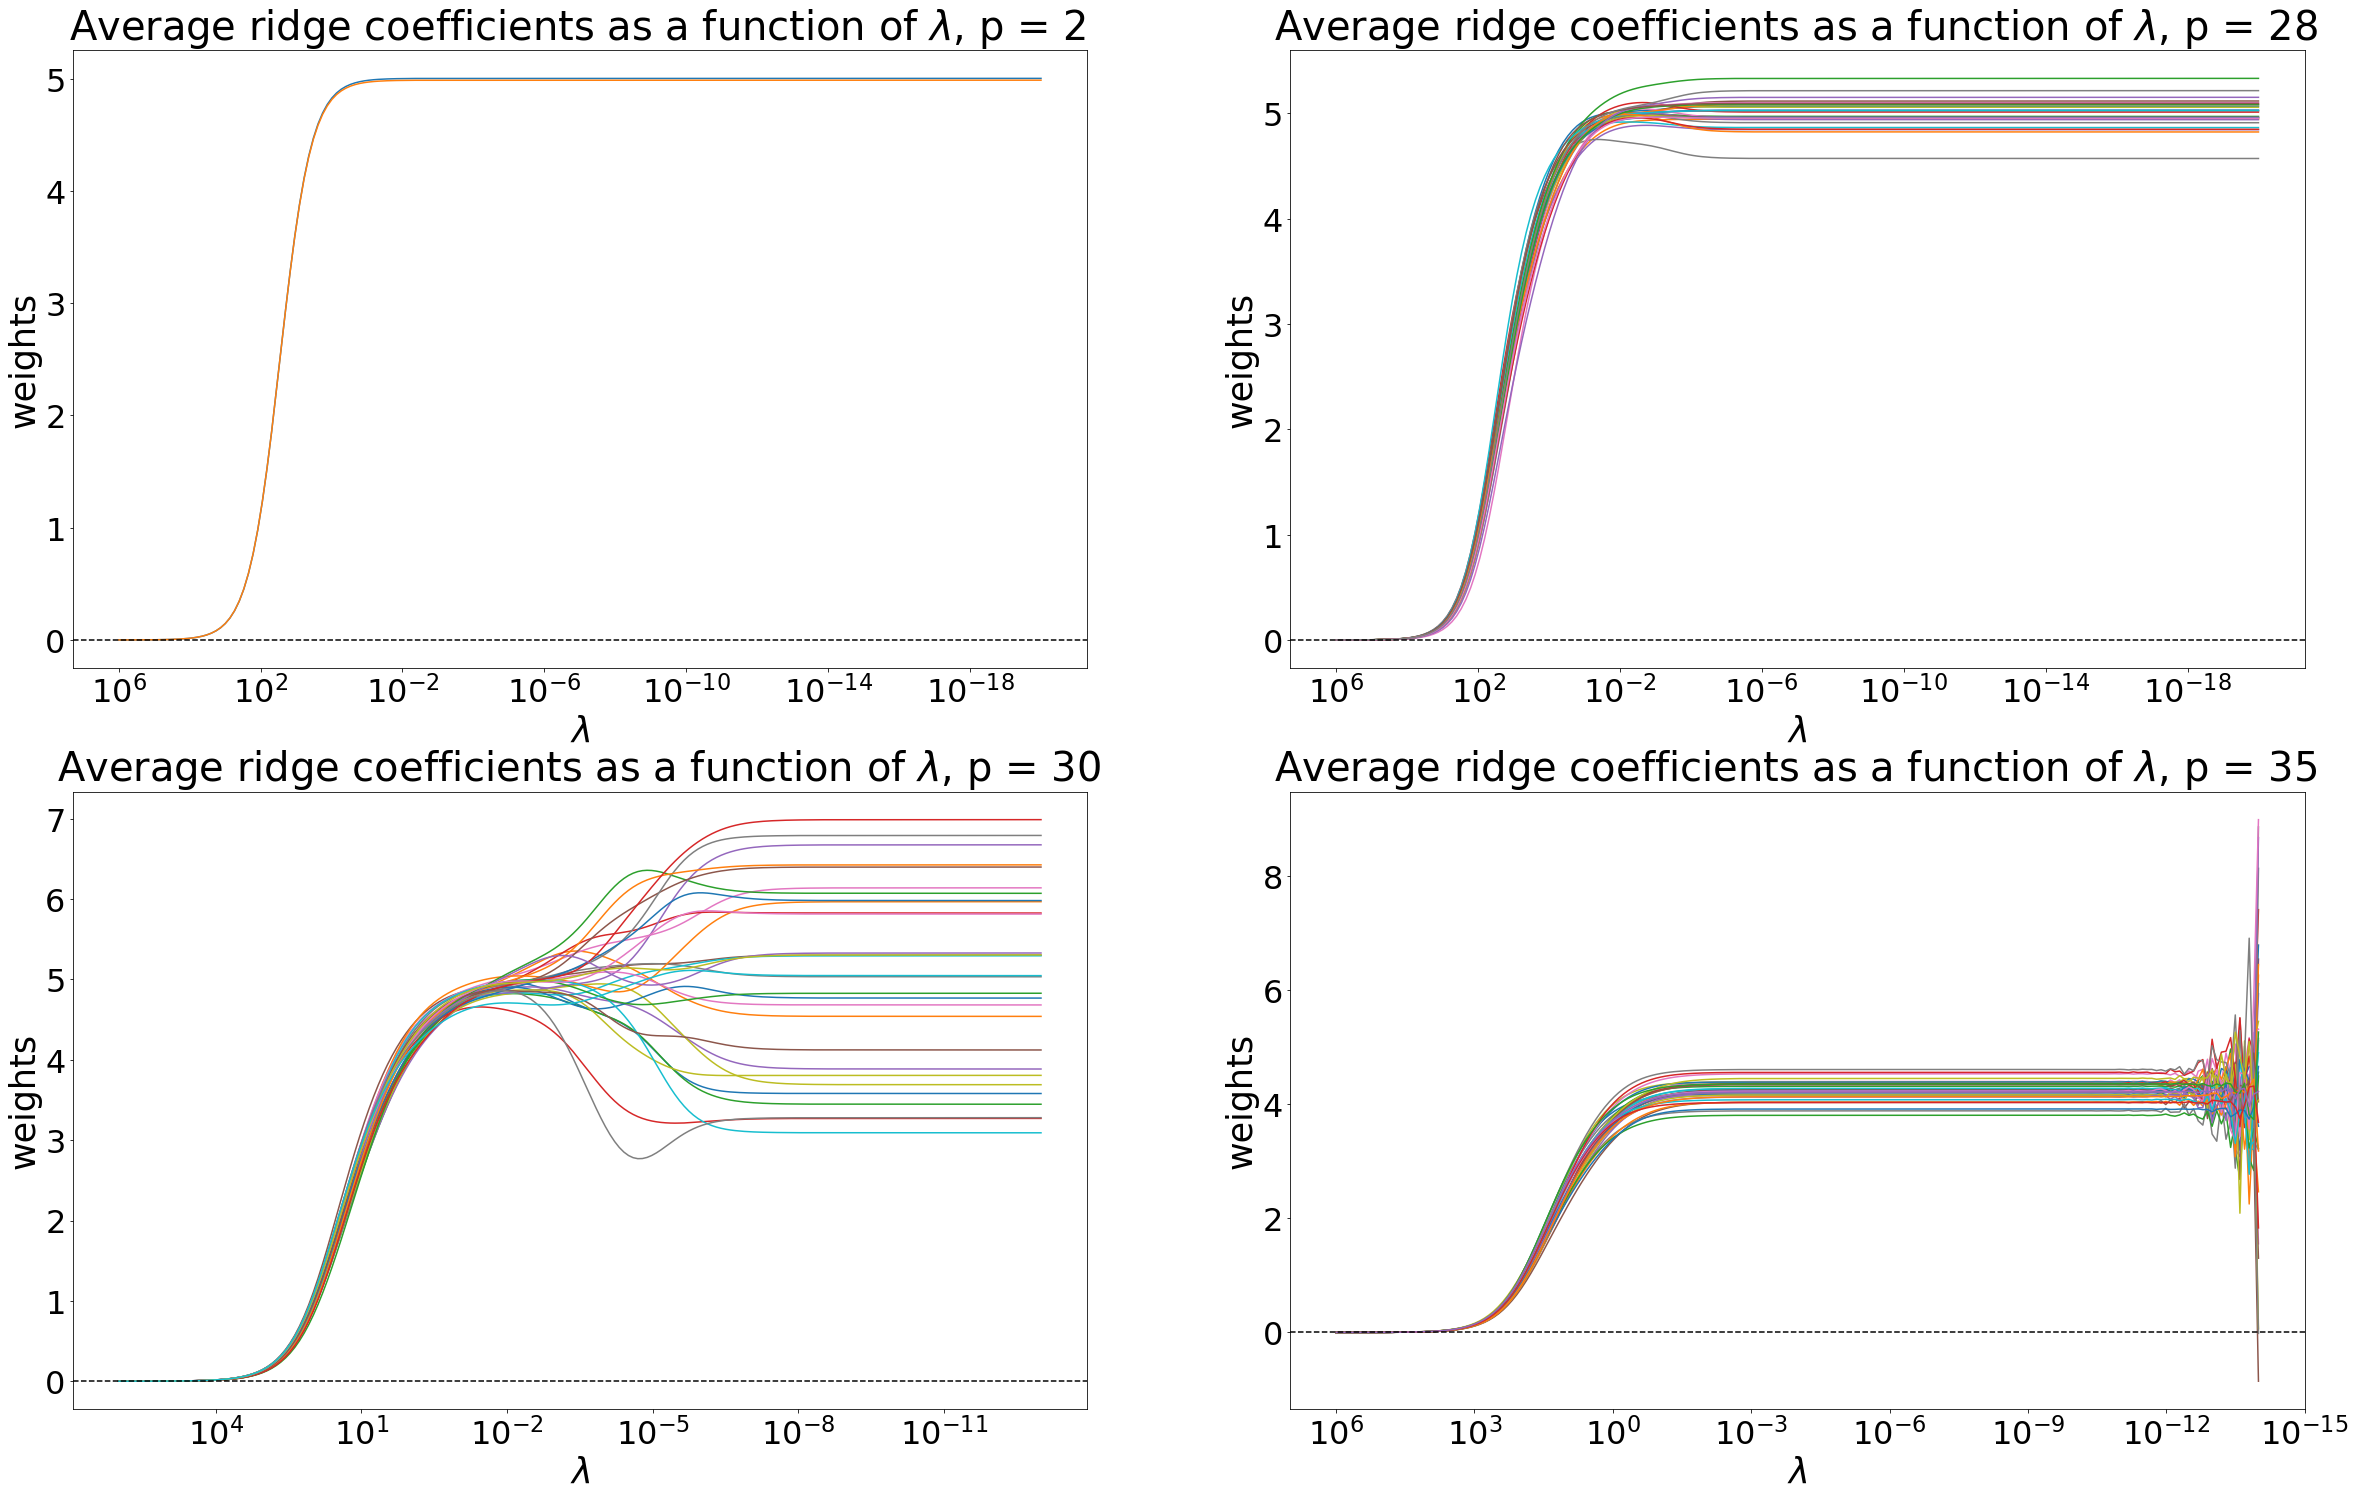
\includegraphics[scale=0.14]{Img/average_ridge_plot_betas.png}
        \centering
    \end{figure}
\end{frame}
%---------------------------------------------------------------------------%
\begin{frame}[fragile]
    \frametitle{Ridge Regression}
    Alternatively,
    \begin{align}
    \label{eqn:eqn2}
    \underset{\beta}{\operatorname{minimize}}\left\{\sum_{i=1}^{n}\left(y_{i}-\beta_{0}-\sum_{j=1}^{p} \beta_{j} x_{i j}\right)^{2}\right\} \text { subject to } \sum_{j=1}^{p}\beta_{j}^{2} \leq t,
    \end{align} \\
    where decreasing values of $t$ indicate an increasingly restrictive optimization constraint. \\
        %are equivalent to small values of $\lambda$.
    Ridge regression yields a closed-form solution for $\beta_{ridge}$:
        \begin{align}
        \label{eqn:eqn3}
        \hat{\beta}_{\lambda}^{R}=\mathbf{Z}_{\lambda} \hat{\beta}=\left(\mathbf{X}^{\prime} \mathbf{X} + \lambda \mathbf{I}\right)^{-1}\left(\mathbf{X}^{\prime} \mathbf{X}\right) \hat{\beta}
        \end{align}
    and for $var(\beta_{ridge})$:
        \begin{align}
        \label{eqn:eqn4}
        V\left(\hat{\boldsymbol{\beta}}_{\lambda}^{R}\right)=\sigma^{2}\left[\mathbf{X}^{\prime} \mathbf{X} + \lambda \mathbf{I}\right]^{-1}\left(\mathbf{X}^{\prime} \mathbf{X}\right)\left[\mathbf{X}^{\prime} \mathbf{X} + \lambda \mathbf{I}\right]^{-1}.
        \end{align}
\end{frame}
%---------------------------------------------------------------------------%
\begin{frame}[fragile]
    \begin{figure}[b]
        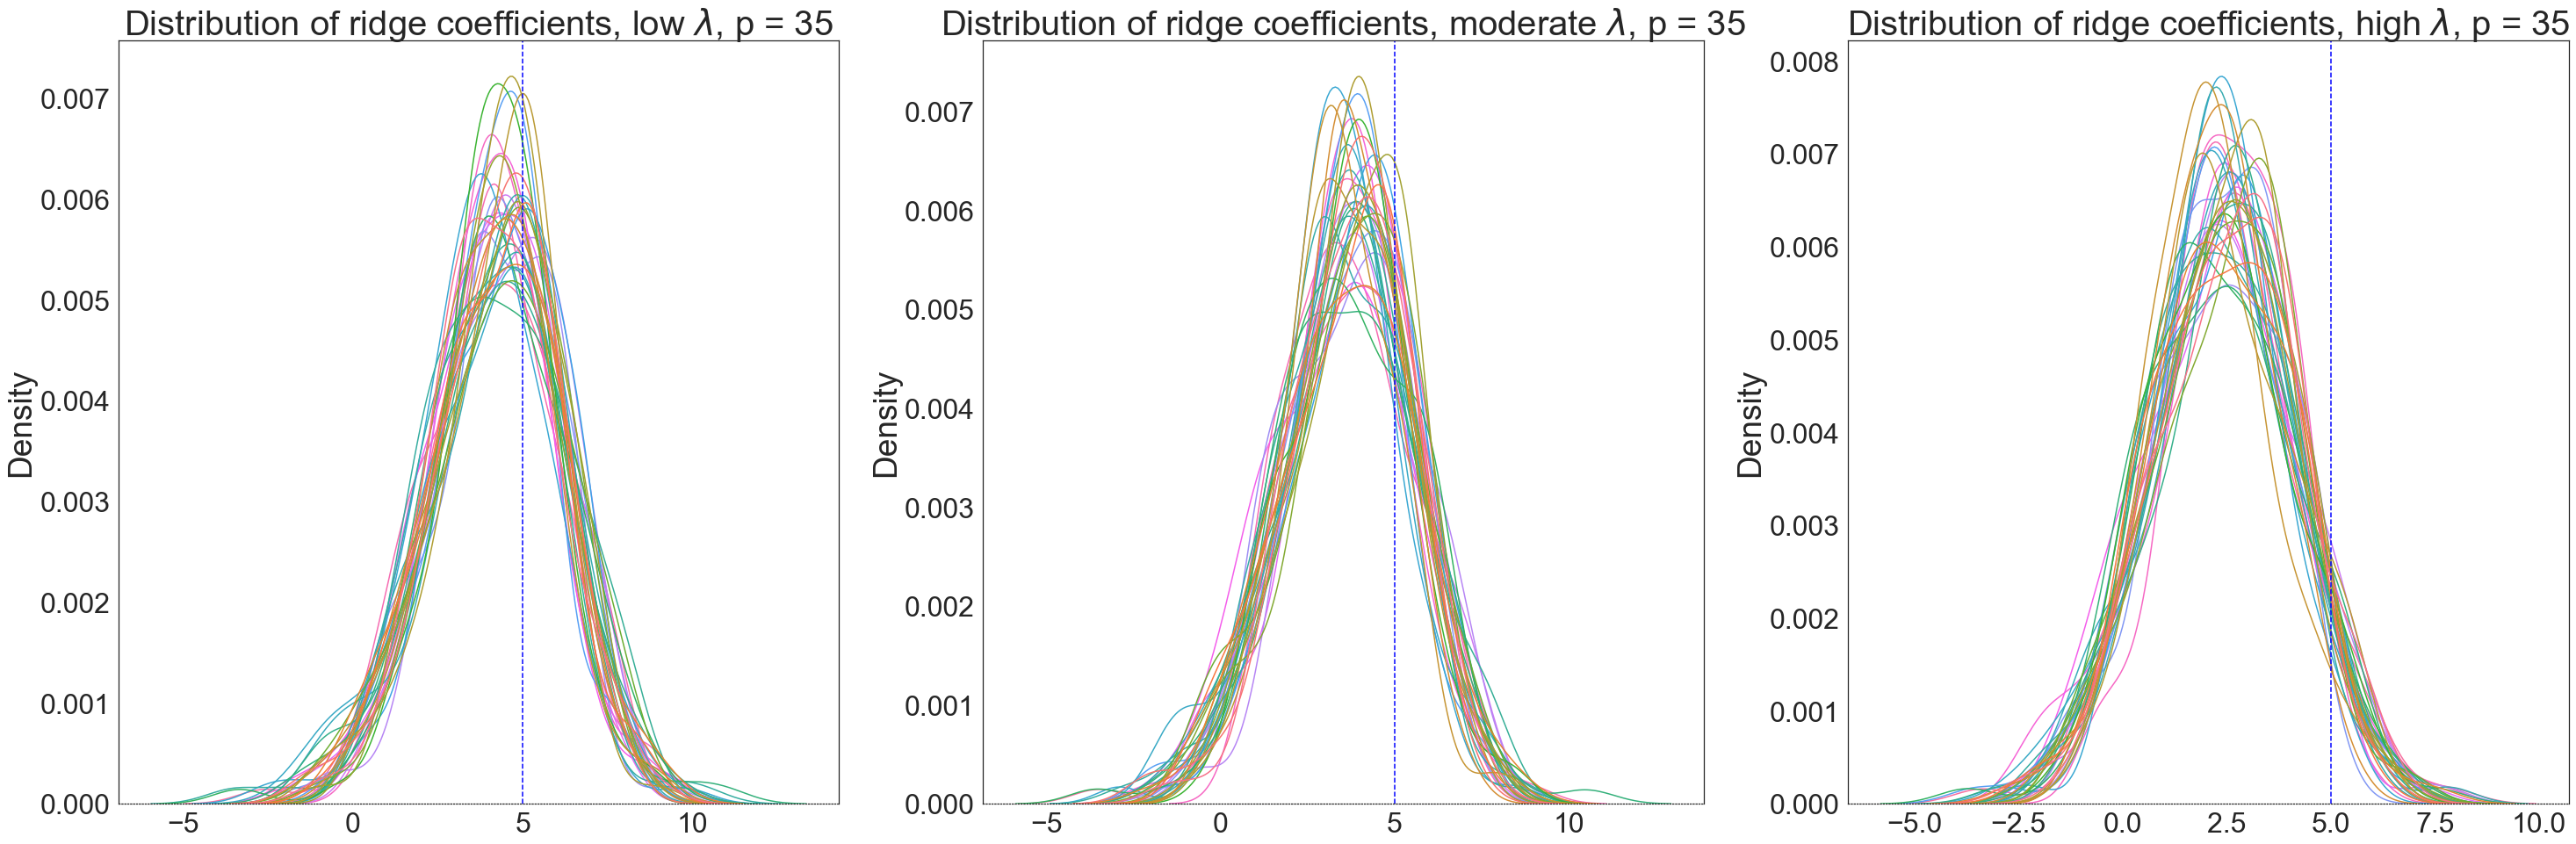
\includegraphics[scale=0.14]{Img/ridge_shrunken_beta_dist_35.png}
        \centering
    \end{figure}
\end{frame}
%---------------------------------------------------------------------------%
\begin{frame}[fragile]
    \frametitle{Lasso Regression}
    Consider the lasso minimization problem, which uses an $\ell_1$-norm constraint:
    \begin{align}
    \label{eqn:eqn5}
    \underset{\beta}{\operatorname{minimize}}\left\{\sum_{i=1}^{n}\left(y_{i}-\beta_{0}-\sum_{j=1}^{p} \beta_{j} x_{i j}\right)^{2}\right\} \text { subject to } \sum_{j=1}^{p}\left|\beta_{j}\right| \leq t,
    \end{align}
    \begin{itemize}
        \item where the $\hat{\beta}_{\lambda}^{L}$ solution is \textit{sparce}: the lasso model holds onto relevant (non-zero) coefficients and sets irrelevant coefficients to \textbf{zero} %(important when $p$ $>$ $n$).
        \item Unlike ridge, lasso is a quadratic programming problem that does not have a closed-form solution.
    \end{itemize}
\end{frame}
%---------------------------------------------------------------------------%
\begin{frame}[fragile]
        \begin{figure}[b]
        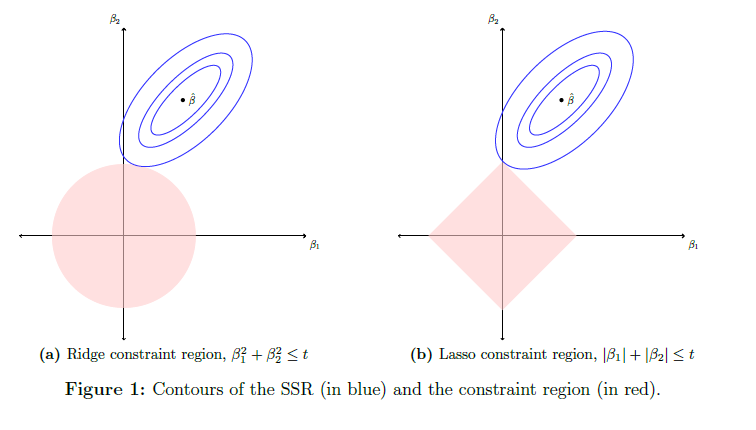
\includegraphics[scale=0.65]{Img/contours.png}\hspace{-1.2cm}
        \centering
    \end{figure}
\end{frame}
%---------------------------------------------------------------------------%
\begin{frame}[fragile]
    \frametitle{Lasso Regression}
    Limitations:
    \begin{itemize}
        \item Degree of sparsity
        \begin{itemize}
            \item Lasso does poorly when a large subset of regressors are $\{j:\beta_j \neq 0\}$ of $\{1,...,p\}$ 
        \end{itemize}
        %\item In the case of grouped multicollinearity, lasso will only select one variable from the group.
            %\begin{itemize}
                %\item Omitted variable bias.
            %\end{itemize}
        \item With high pairwise correlation among predictors, ridge regression outperforms lasso in terms of prediction.
        \item Lasso can only select up to $n$ regressors when $p$ > $n$.
    \end{itemize}
\end{frame}
%---------------------------------------------------------------------------%
\begin{frame}[fragile]
    \begin{figure}[b]
        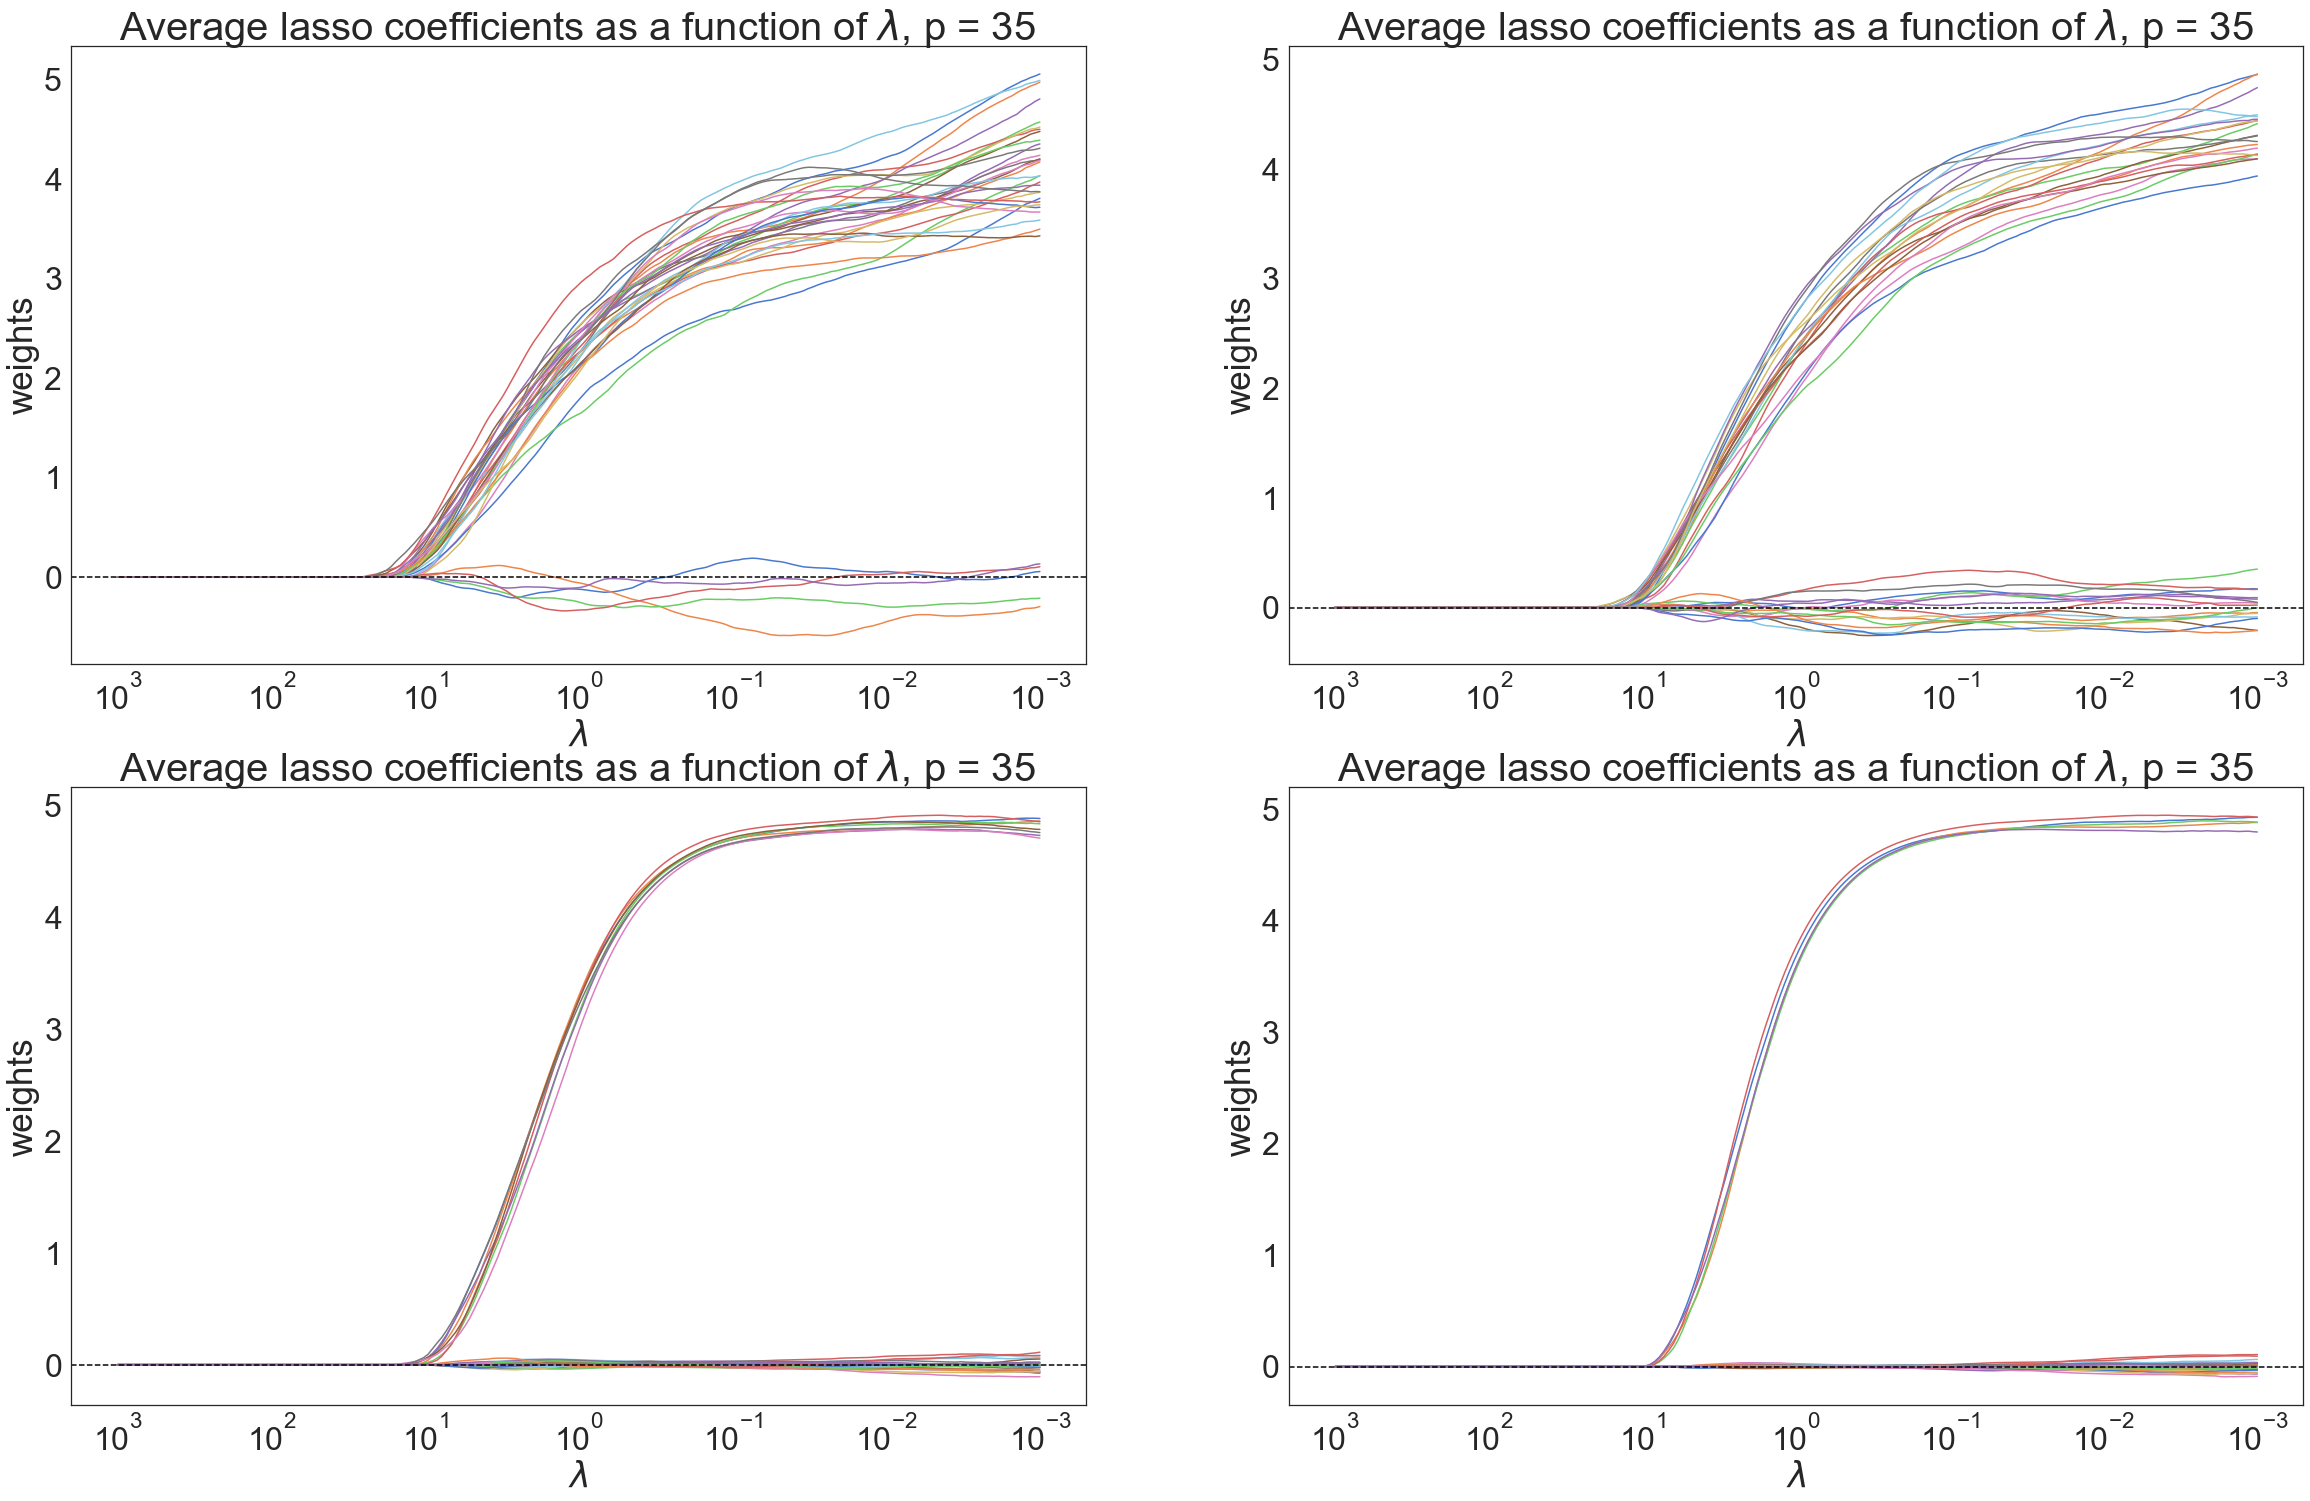
\includegraphics[scale=0.14]{Img/average_lasso_plot_betas.png}
        \centering
    \end{figure}
\end{frame}
%---------------------------------------------------------------------------%
\begin{frame}[fragile]
%\frametitle{Variance-Bias Tradeoff}
    \begin{figure}[b]
        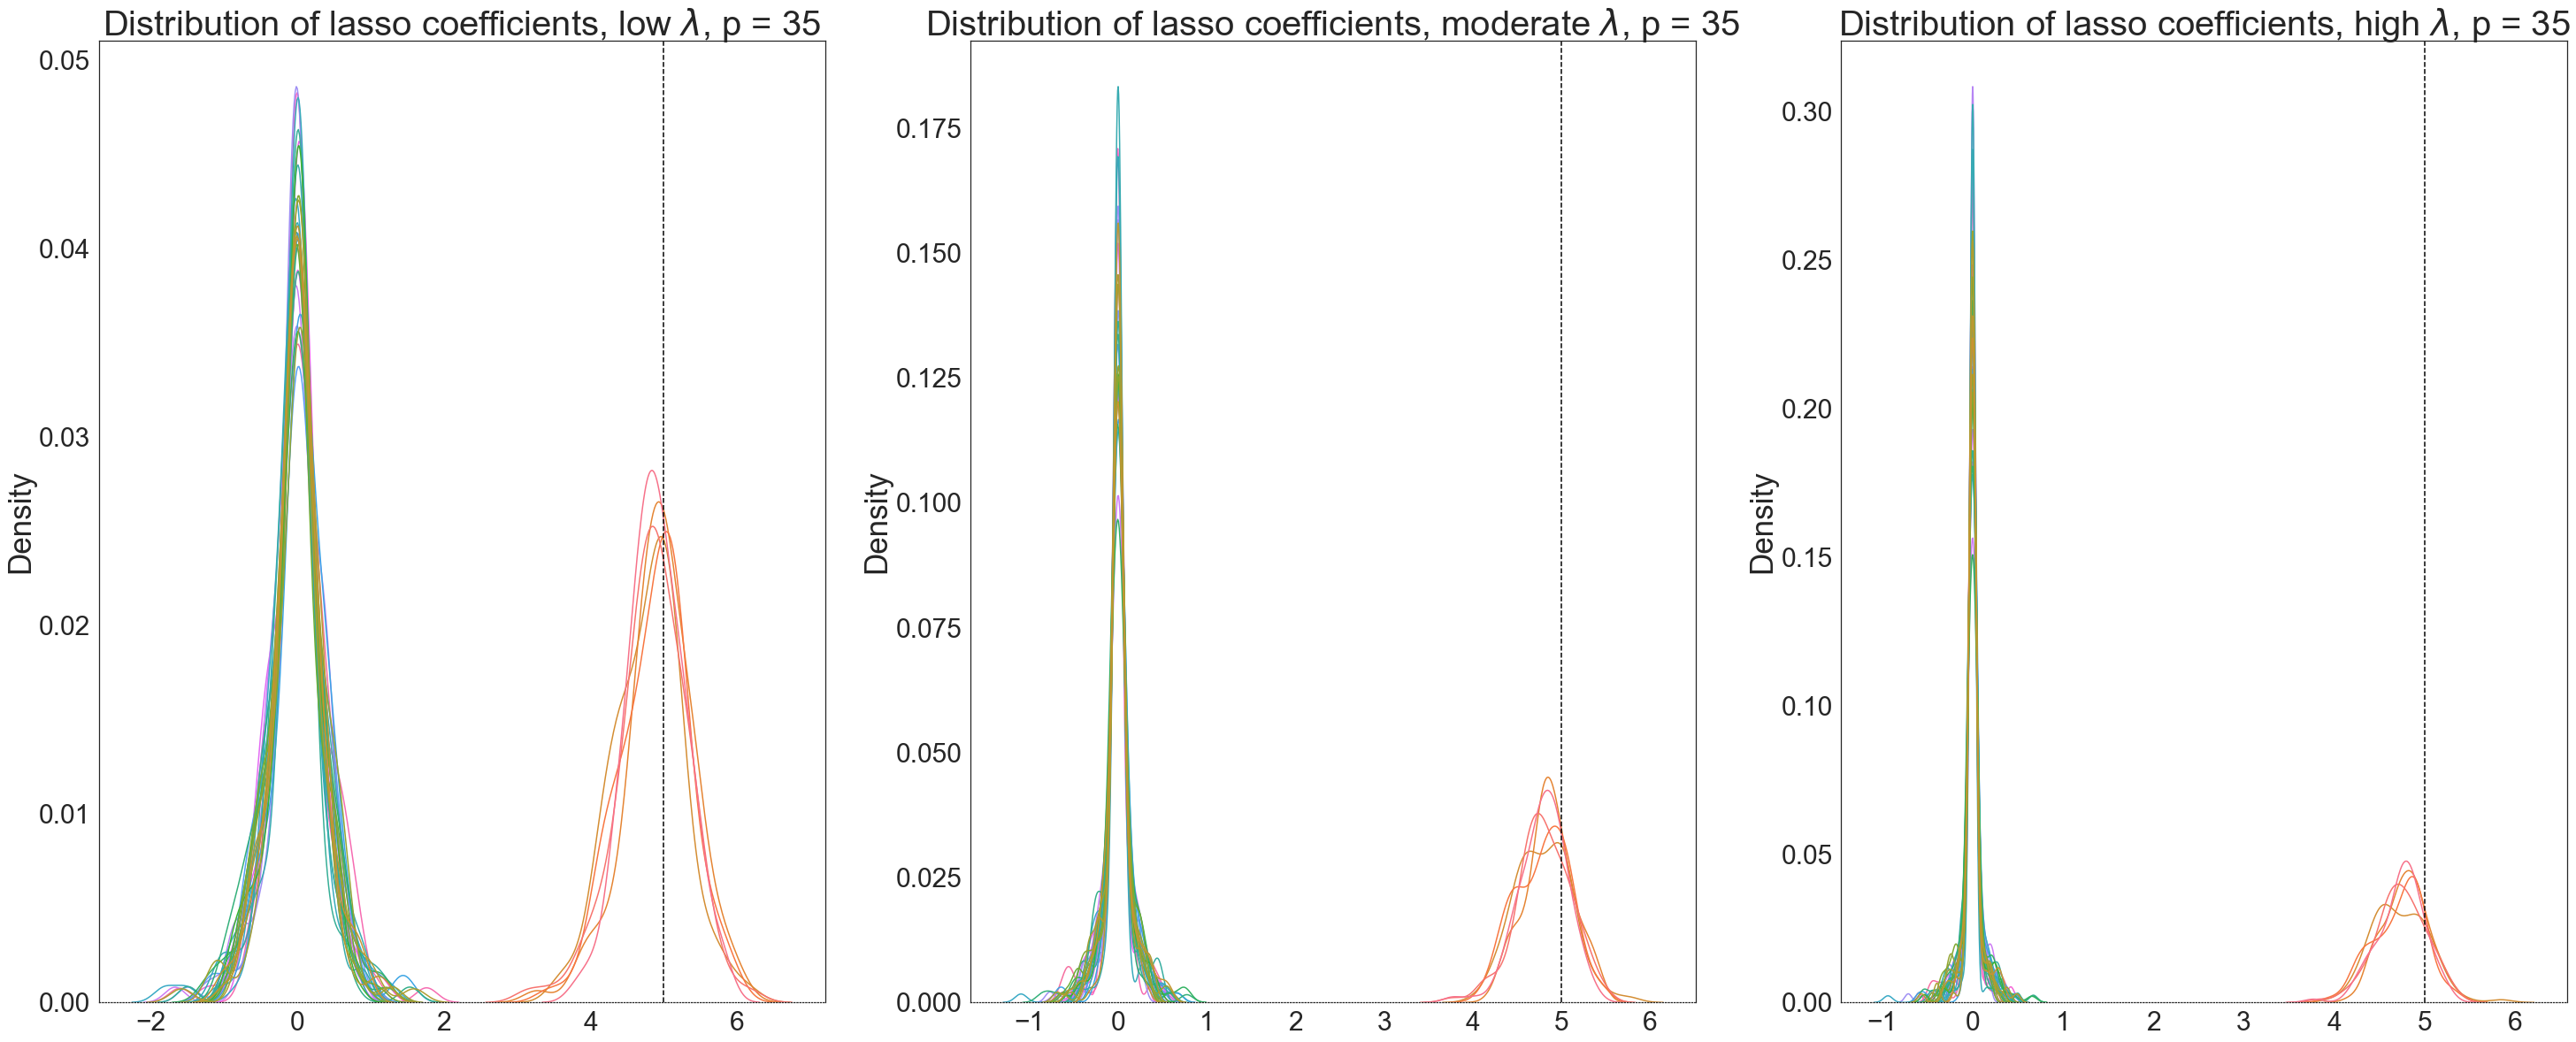
\includegraphics[scale=0.15]{Img/lasso_shrunken_beta_dist_35.png}
        \centering
    \end{figure}
\end{frame}
%---------------------------------------------------------------------------%
\begin{frame}[fragile]
    \frametitle{"Naïve" Elastic Net Regression}
    Consider the "naïve" elastic net minimization problem, which is subject to a constraint that is represented as a convex combination of the ridge and lasso shrinkage penalties:
    \begin{align}
    \label{eqn:eqn6}
    \underset{\beta}{\operatorname{minimize}}\left\{\sum_{i=1}^{n}\left(y_{i}-\beta_{0}-\sum_{j=1}^{p} \beta_{j} x_{i j}\right)^{2}\right\} \text { subject to } \left(1 - \alpha \right)\sum_{j=1}^{p}\left|\beta_{j}\right| + \alpha \sum_{j=1}^{p}\beta_{j}^{2} \leq t
    \end{align}
    where $\alpha$ represents the weight assigned to the ridge penalty. 
    %where $\alpha = \lambda_{2} / \left(\lambda_{1} + \lambda_{2}\right)$ .
    \begin{itemize}
        \item Contains the best features of ridge and lasso regression (continuous shrinkage and simultaneous variable selection).
        \begin{itemize}
            \item For all $\alpha \in [0, 1)$, the elastic net penalty function is singular at 0 and strictly convex for all $\alpha > 0$.
            \item Strict convexity is what sets elastic net apart from lasso.
        \end{itemize}
    \end{itemize}
\end{frame}
%---------------------------------------------------------------------------%
\begin{frame}[fragile]
    \frametitle{"Naïve" Elastic Net Regression}
    \begin{itemize}
        \item \textbf{Improves over the lasso by}
            \begin{itemize}
                \item overcoming the saturation of variable selection when $p > n$. \textbf{(variable selection)}
                \item accounting for highly correlated "grouped" variables. \textbf{(continuous shrinkage)}
                \item strengthening prediction performance if substantial multicollinearity among predictors exists in cases where $n > p$.
            \end{itemize}
        %\item Intuition: for each fixed $\lambda$ we find ridge coefficients and then lasso coefficients.
        \item \textbf{Limitations}
            \begin{itemize}
                \item Double shrinkage does not reduce variance and unnecessarily introduces added bias.
                \item Hence, works only when its solution is very close to either ridge or lasso.
            \end{itemize}
    \end{itemize}
\end{frame}
%---------------------------------------------------------------------------%
\begin{frame}[fragile]
    \frametitle{Elastic Net Regression}
    Given the data set (y,X) and the two fixed non-zero Lagrangian parameters, ($\lambda_{1}$,$\lambda_{2}$), derived from the naïve elastic net's optimization problem, \emph{Lemma 1} of \cite{zou2005regularization} defines the artificial data set ($\mathbf{y}^*$, $\mathbf{X}^*$): 
    
    \begin{align}
        \label{eqn:eqn7}
            \hat{\beta}^*=\arg \min_{\hat{\beta}^*}|\mathbf{y}^* - \mathbf{X}^*\beta^*|^2 + \frac{\lambda_1}{\sqrt{(1+\lambda_2)}}|\beta^*|_{1}
    \end{align}
    
    With the corrected elastic net estimates $\hat{\beta}$ defined as 
    \begin{align}
        %\label{eqn:eqn8}
            \hat{\beta}(elastic \: net)=\sqrt{(1+\lambda_2)}\hat{\beta^*}
    \end{align}
    and 
    \begin{align}
        %\label{eqn:eqn9}
            \hat{\beta}(naive \: elastic \: net)={1 / \sqrt{(1+\lambda_2)}}\hat{\beta^*}
    \end{align}
    
    Finally,
    \begin{align}
        \label{eqn:eqn10}
            \hat{\beta}(elastic \: net)=(1+\lambda_2)\hat{\beta}(naive \: elastic \: net). 
    \end{align}
\end{frame}
%---------------------------------------------------------------------------%
\begin{frame}[fragile]
    \begin{figure}[b]
        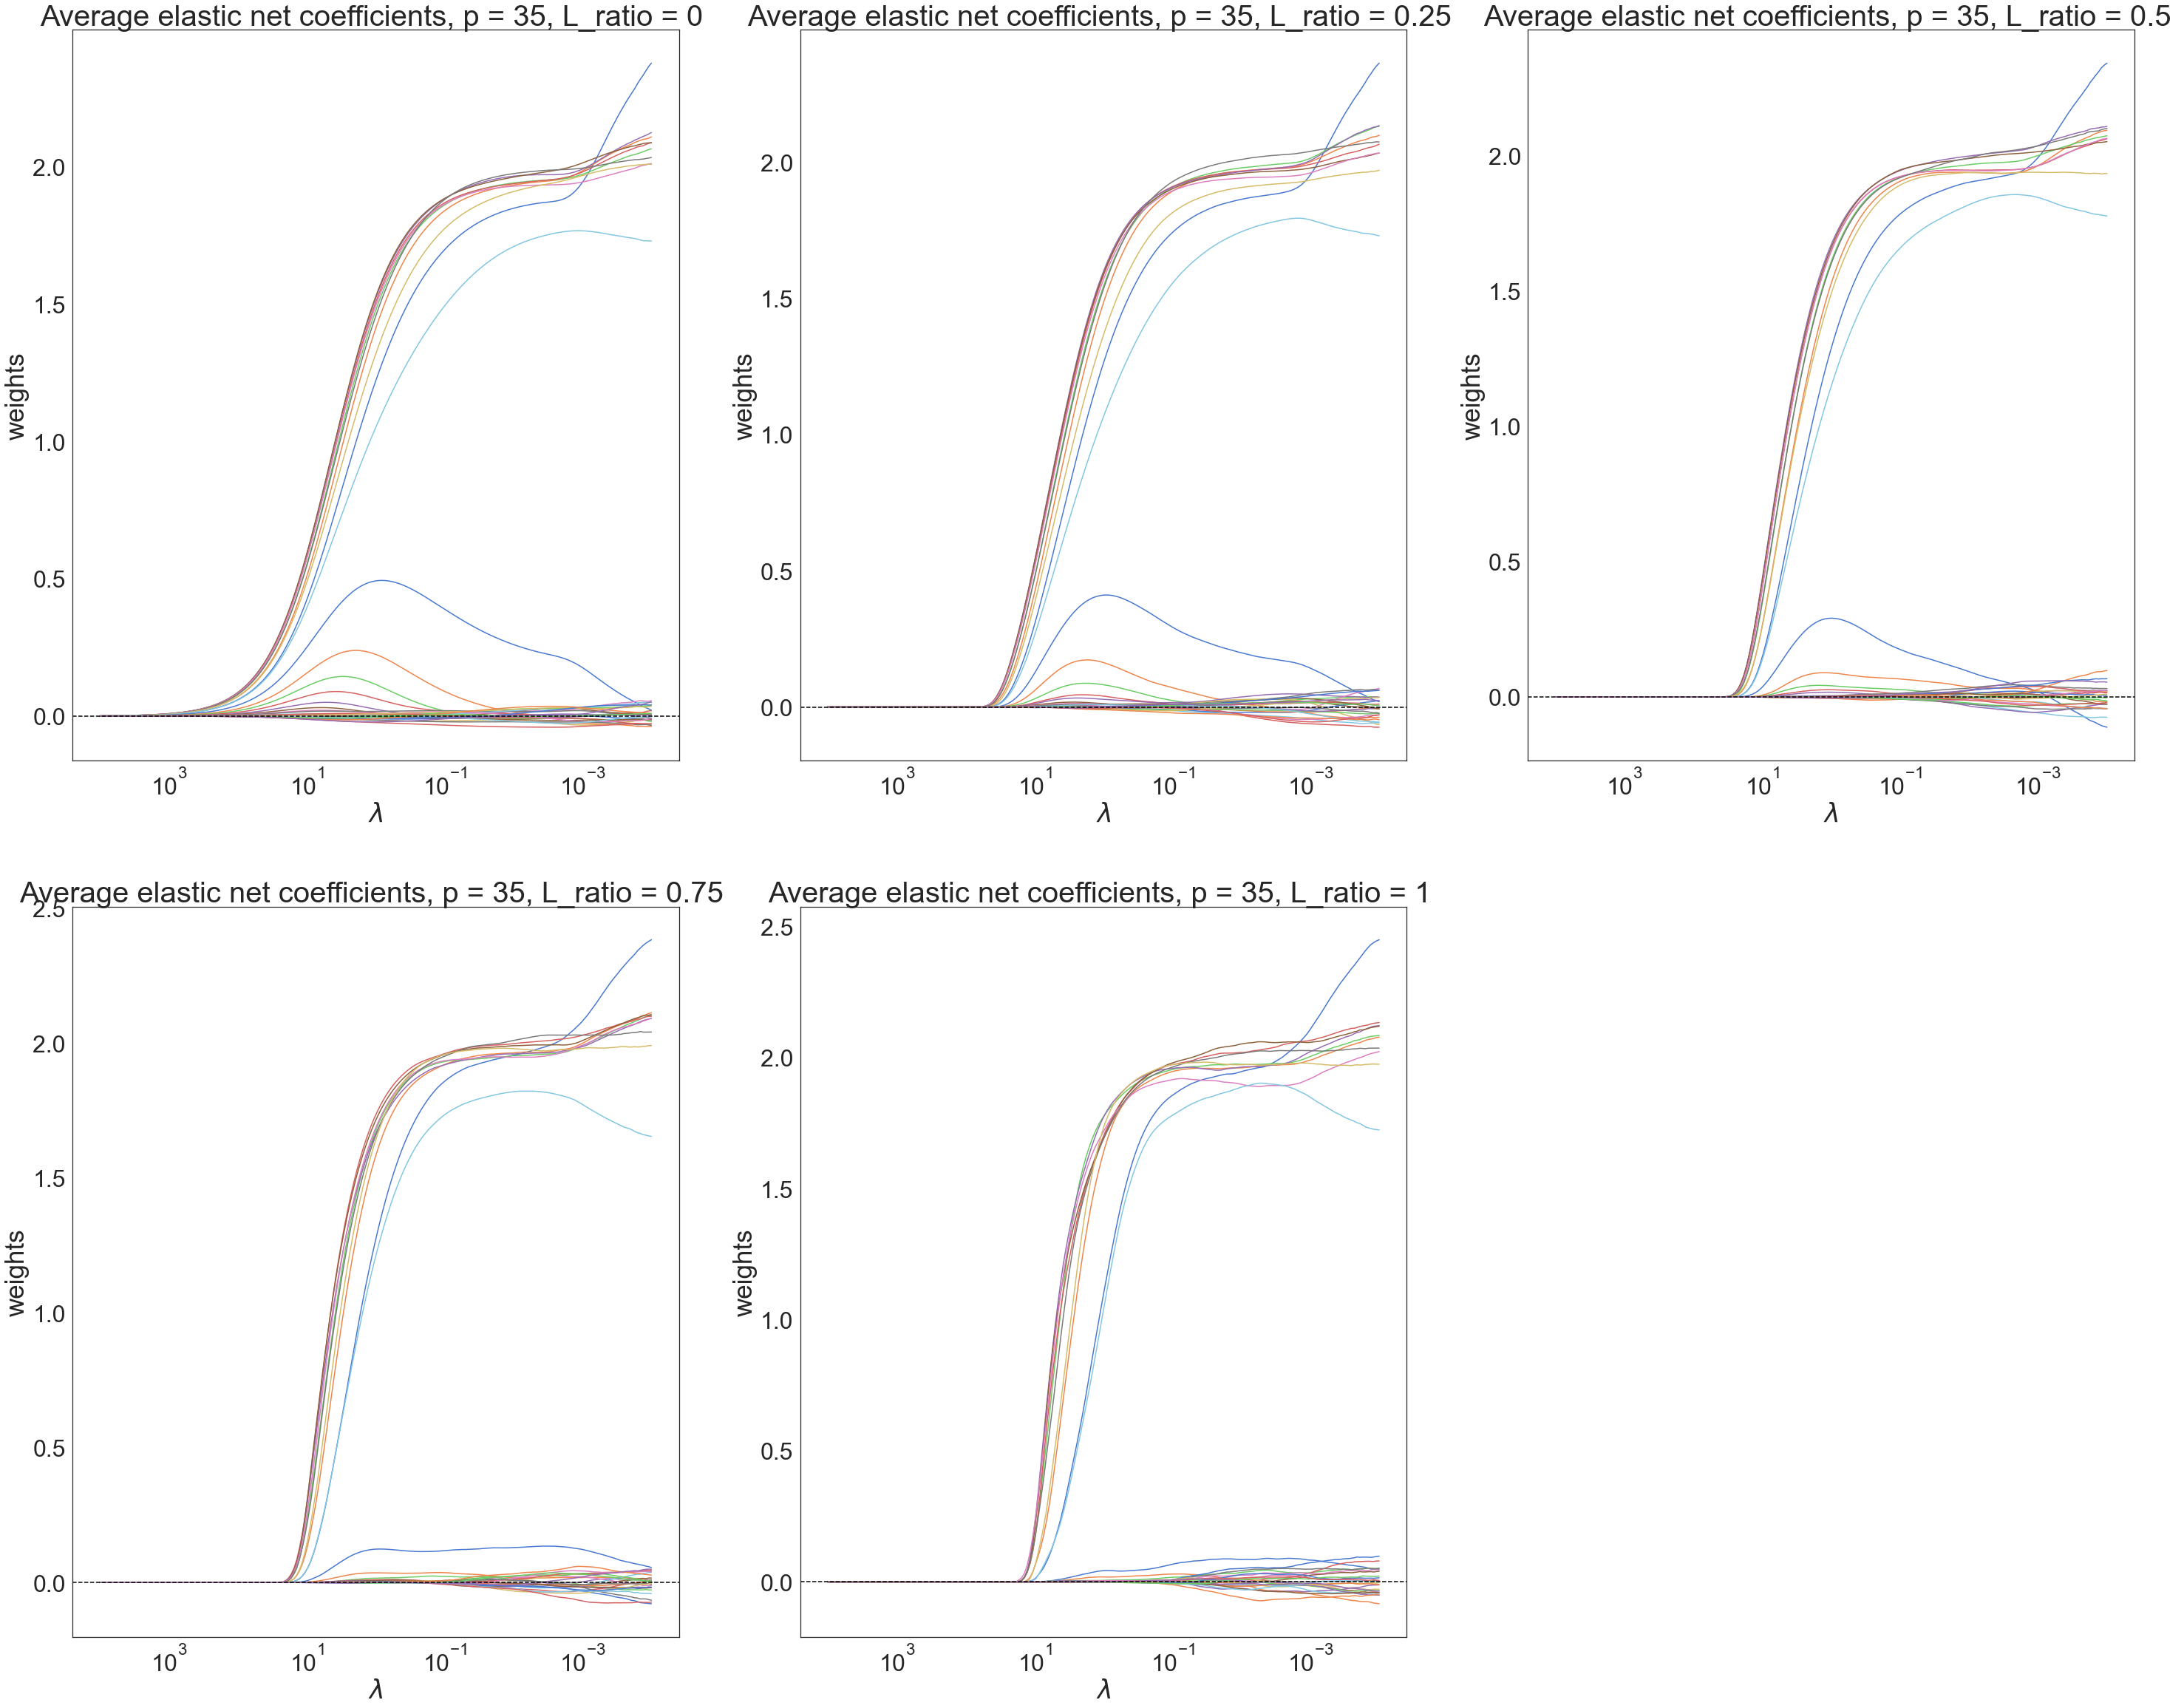
\includegraphics[scale=0.095]{Img/elastic_net_plot_average_betas.png}
        \centering
    \end{figure}
\end{frame}
%---------------------------------------------------------------------------%
\begin{frame}[fragile]
    \begin{figure}[b]
        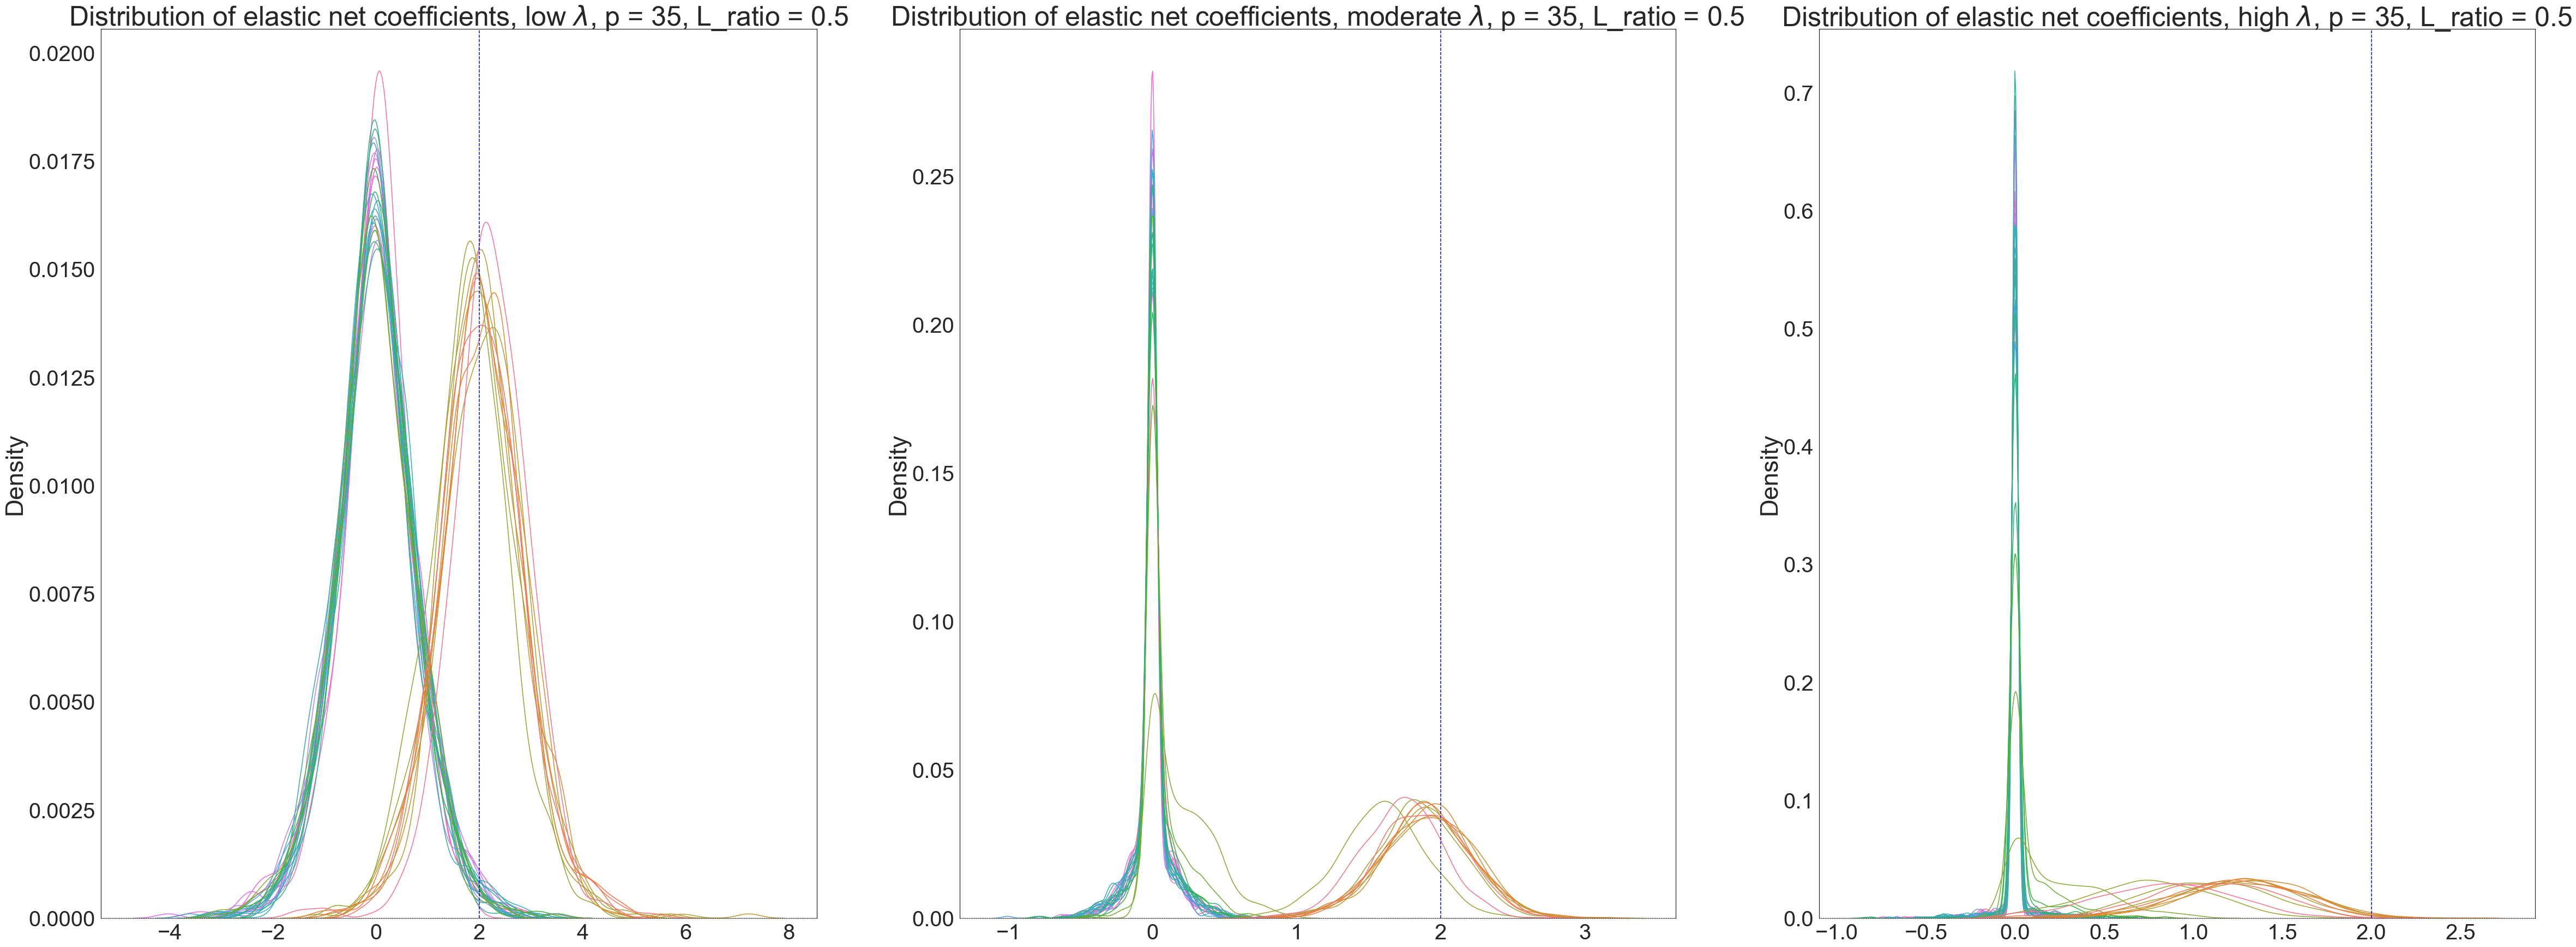
\includegraphics[scale=0.09]{Img/elastic_net_shrunken_beta_dist_35_0.5.png}
        \centering
    \end{figure}
\end{frame}
%---------------------------------------------------------------------------%
\begin{frame}[fragile]
\frametitle{Regularization Methods Summarized}
\tiny
\begin{table}
\begin{tabular}[h]{ ||m{2cm}|m{5cm}|m{5cm}||  }
\hline
Model & Characteristics & Drawbacks \\
\hline\hline
Ridge
& 
\begin{itemize}
    \item $\ell_2$-norm shrinkage penalty %($\hat{\beta} \rightarrow 0$)
    \item Performs well in the presence of multicollinearity.
\end{itemize}
& 
\begin{itemize}
    \item Does not perform variable selection.
\end{itemize} \\
\hline
Lasso
& 
\begin{itemize}
    \item  $\ell_1$-norm shrinkage penalty %($\hat{\beta} = 0$)
    \item Performs variable selection.
\end{itemize}
& 
\begin{itemize}
    \item Does not behave well when sparsity is very low.
    \item Cannot handle high correlation or grouped multicollinearity. 
    \item Can only select up to $n$ regressors when $p > n$
\end{itemize} \\
\hline
Naïve Elastic Net
& 
\begin{itemize}
    \item  convex combination of $\ell_1$-norm and $\ell_2$-norm shrinkage penalties. 
    \item Potentially selects all $p$ in the presence of grouped collinearity.
\end{itemize}
& 
\begin{itemize}
    \item Double shrinkage does not contribute to further reduction of the variances and adds unnecessary bias.
    \item Works only when solution is very close to ridge or lasso.
\end{itemize} \\
\hline
Elastic Net
&
\begin{itemize}
    \item Maintains all characteristics from naïve model, but corrects for double shrinkage.
\end{itemize}
&
\tabularnewline
\hline
\end{tabular}
% \caption{Summary of methodologies}
% \label{table:1}
\end{table}
\end{frame}
%---------------------------------------------------------------------------%
%\begin{frame}
%\begin{columns}[t]
%\column{.5\textwidth}
%\centering
%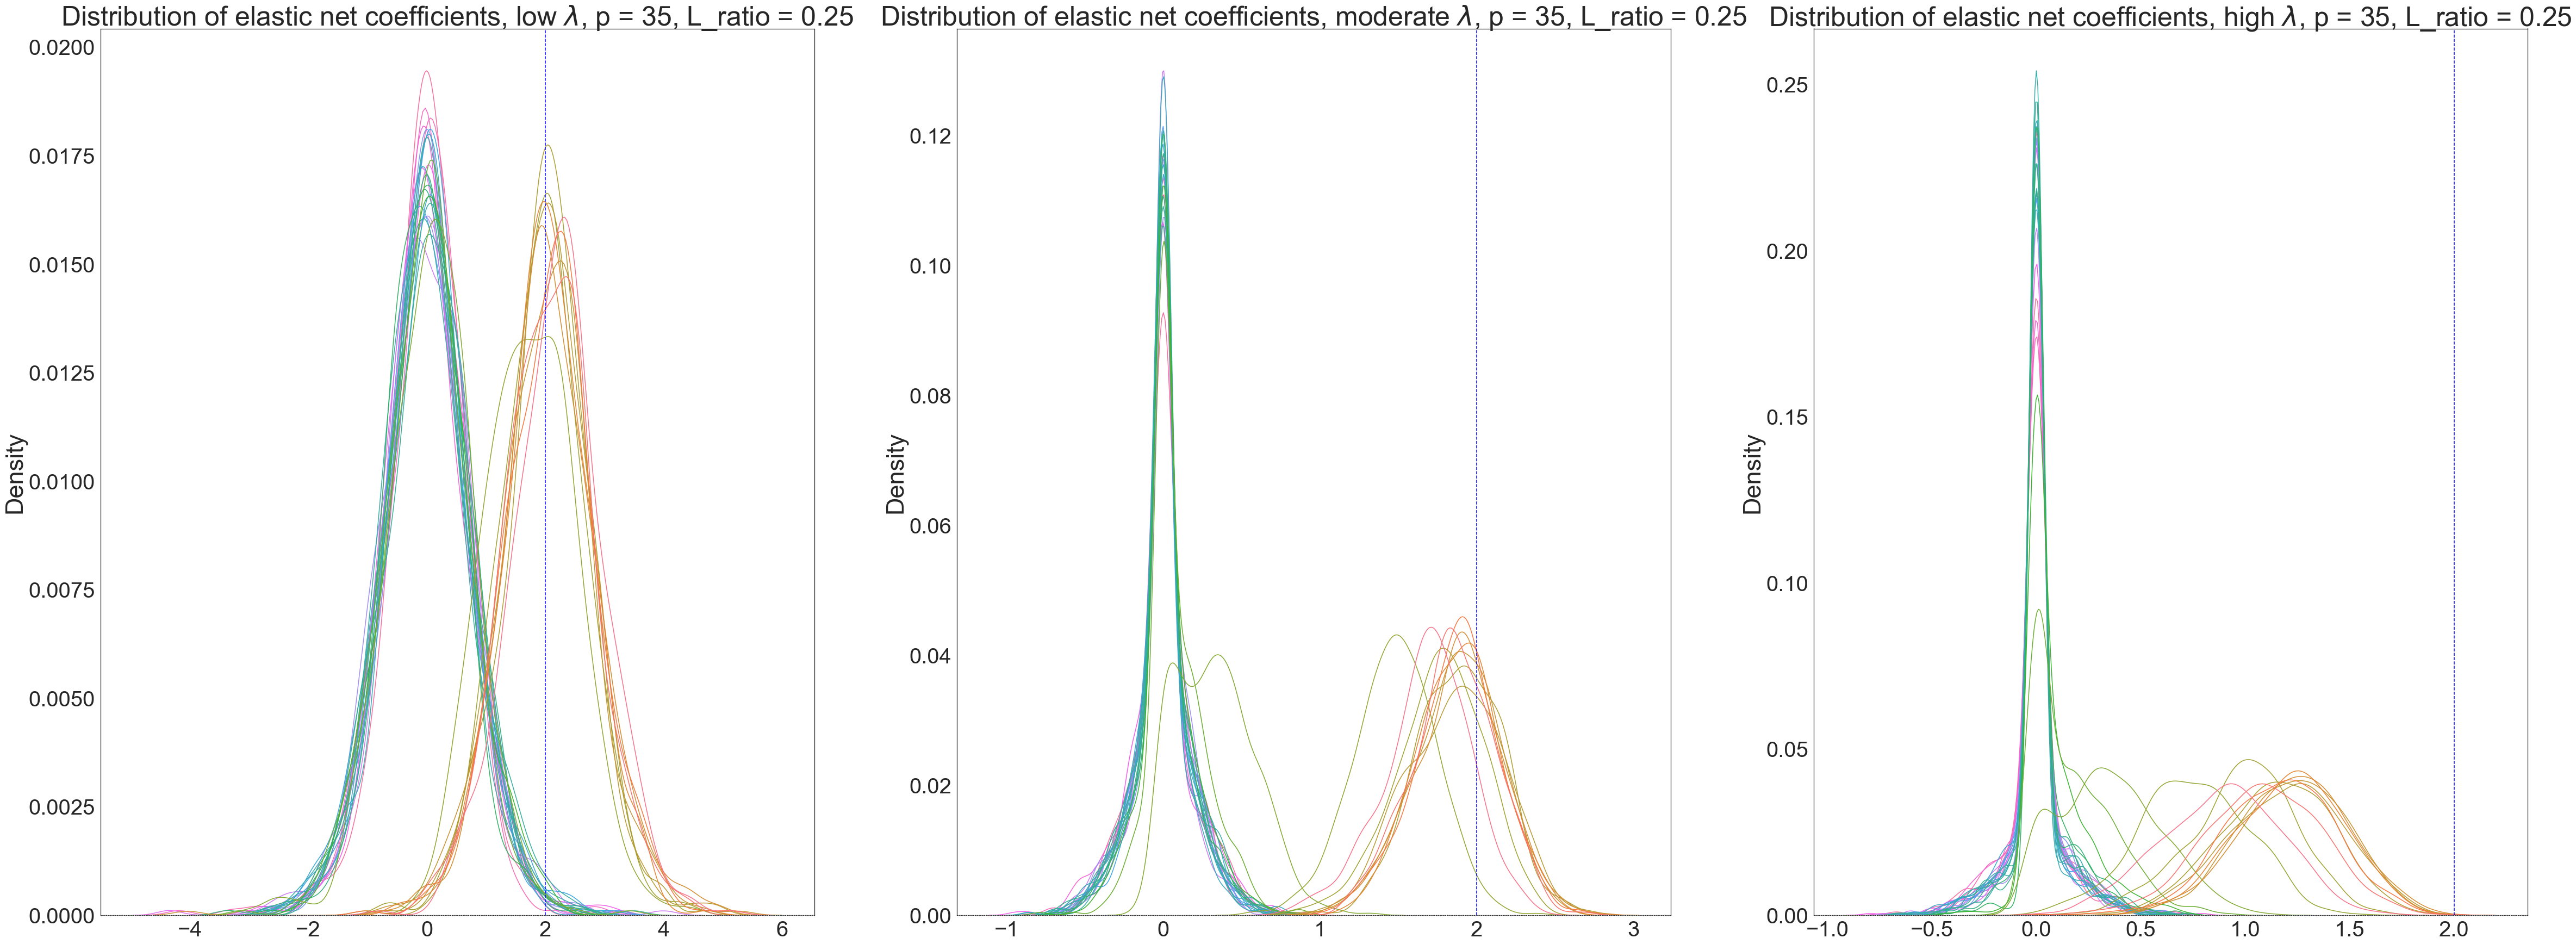
\includegraphics[width=7cm,height=4cm, left]{Img/elastic_net_shrunken_beta_dist_35_0.25.png}
%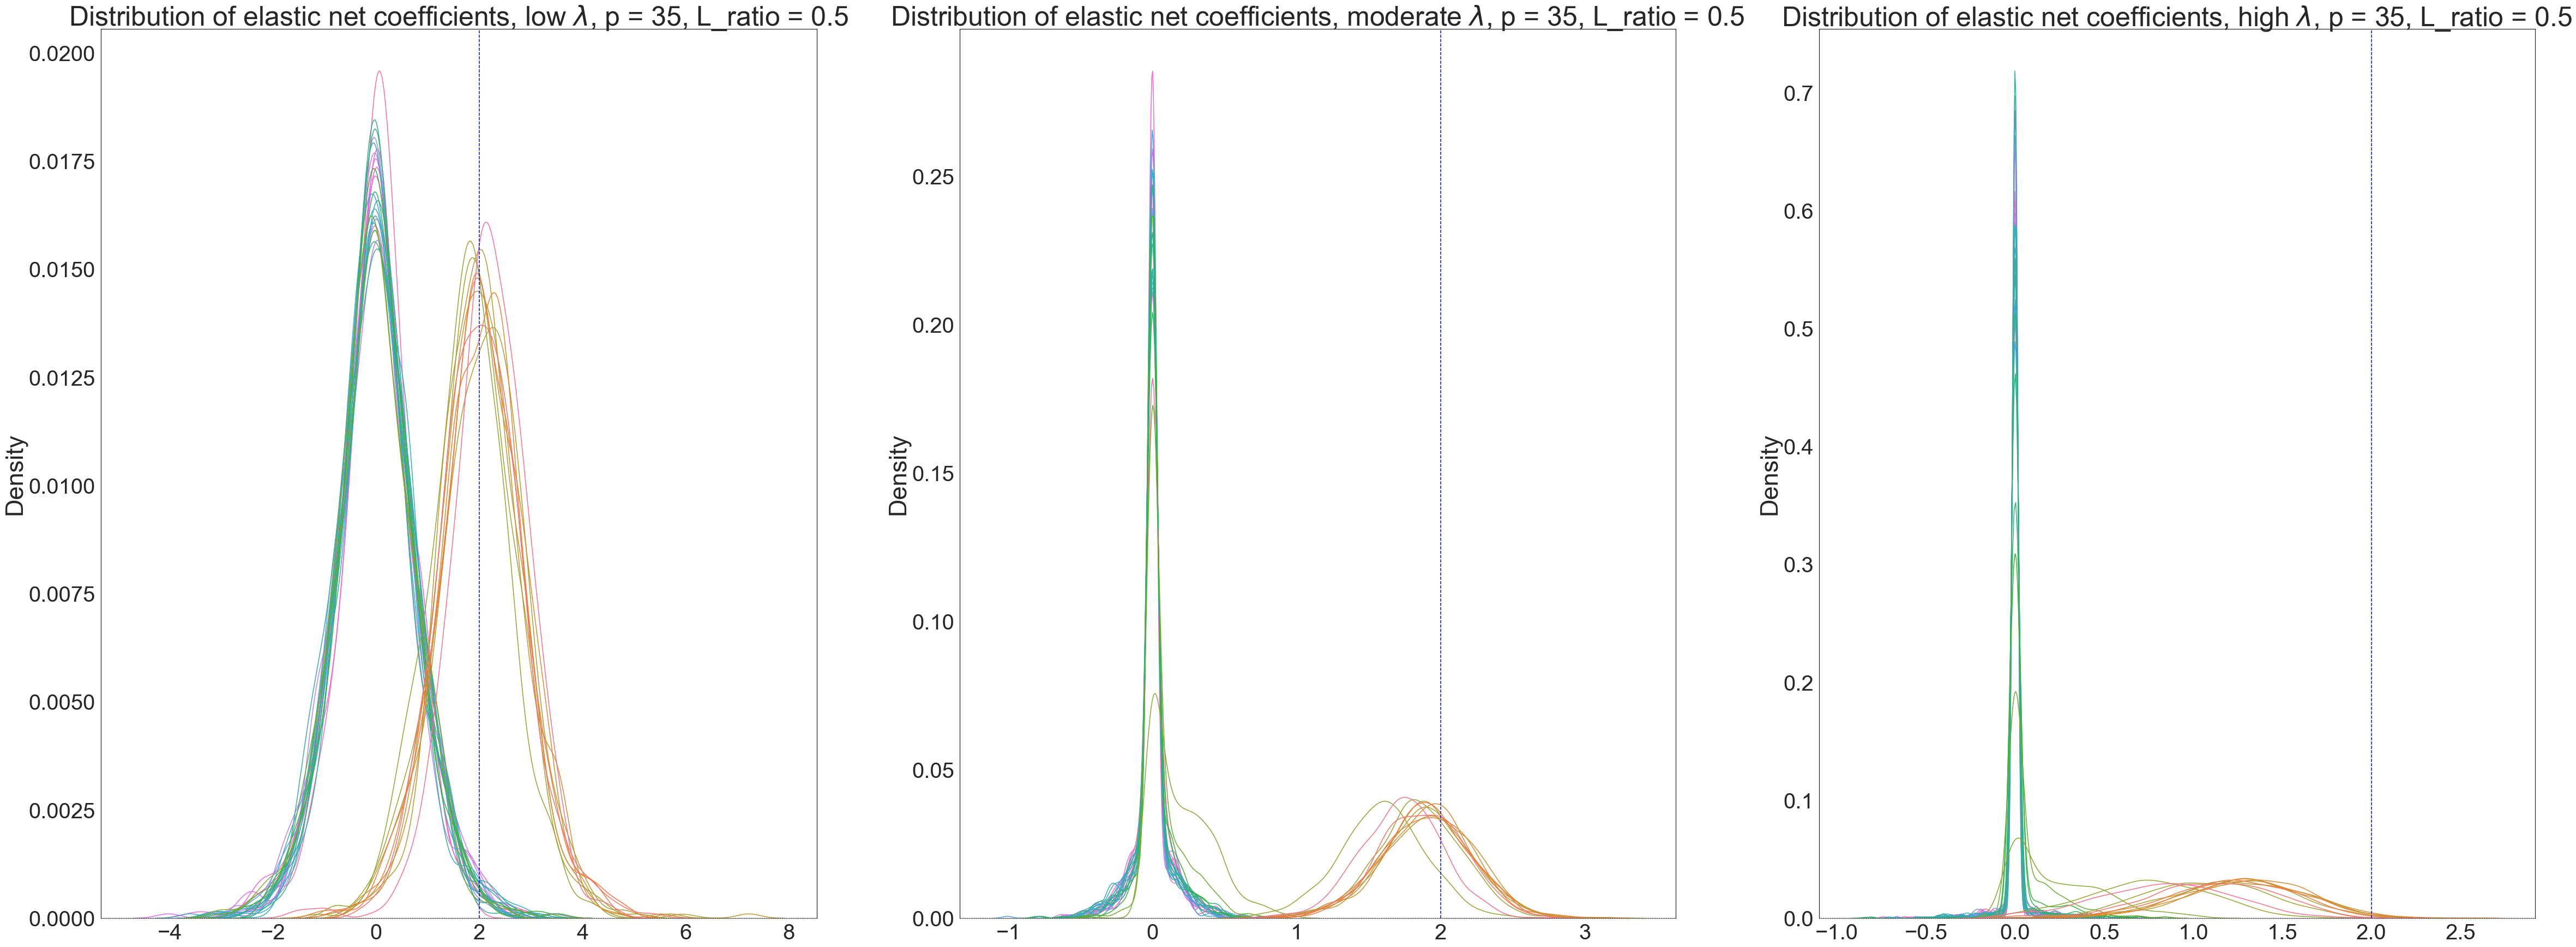
\includegraphics[width=7cm,height=4cm, right]{Img/elastic_net_shrunken_beta_dist_35_0.5.png}\\
%\column{1.0\textwidth}
%\centering
%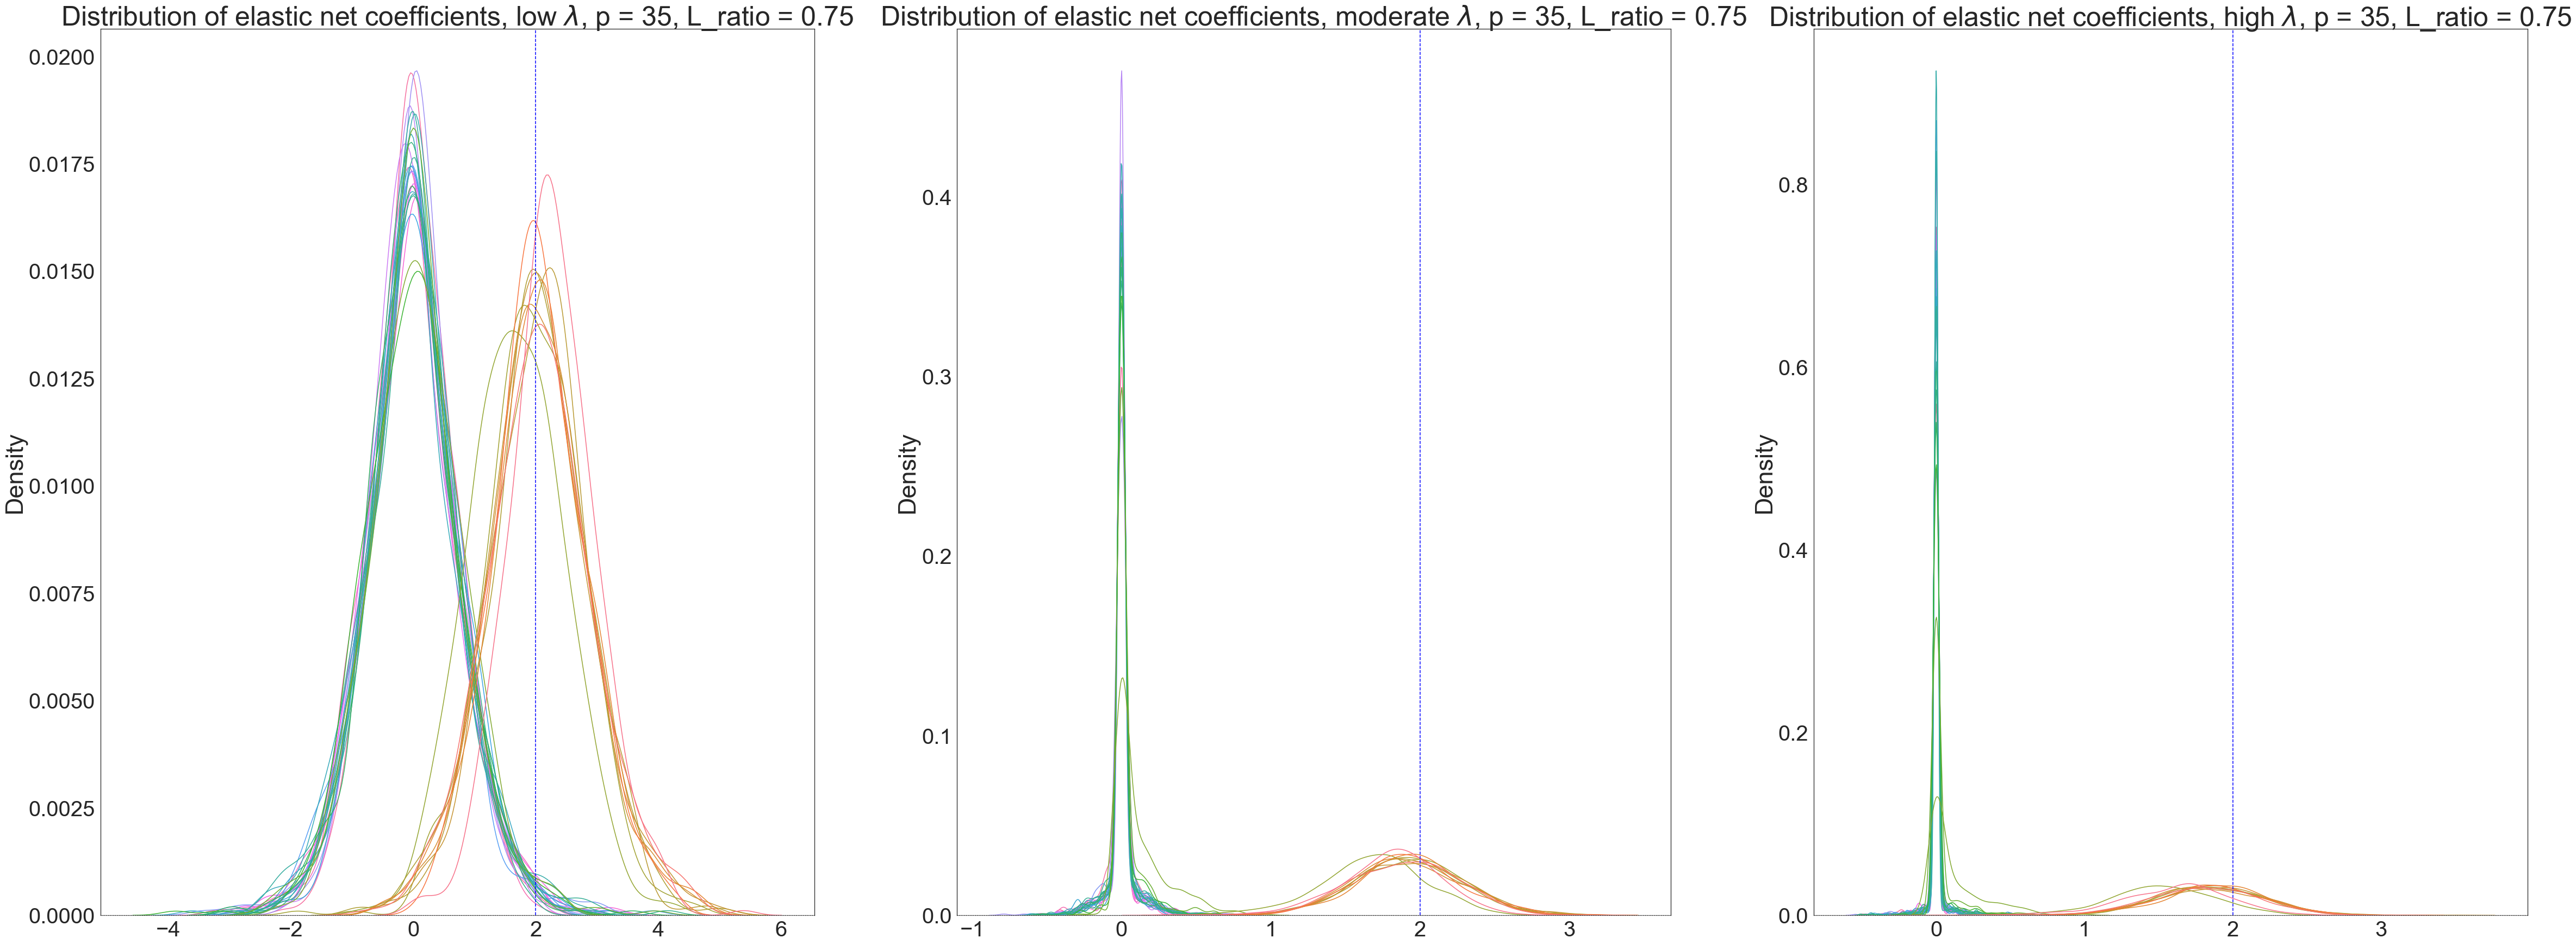
\includegraphics[width=7cm,height=4cm, center]{Img/elastic_net_shrunken_beta_dist_35_0.75.png}\\
%\end{columns}
%\end{frame}
%---------------------------------------------------------------------------%
%->> Simulation
%---------------------------------------------------------------------------%
%---------------------------------------------------------------------------%
\lecture{Research Presentation}{lec_present_sim}
%---------------------------------------------------------------------------%
\section{Simulation study}%
%---------------------------------------------------------------------------%
\begin{frame}[fragile]
    \frametitle{Measuring Prediction Performance}
    \begin{itemize}
        \item Selects the model that best fits the data.
        \item Bias-Variance Decomposition
        \begin{itemize}
            \item We carefully follow \cite{hastie2008elements}.
            \item Assume $Y=f(X) + \varepsilon$, where $E[\varepsilon]=0$ and $Var(\varepsilon)=\sigma^2_{\varepsilon}$
            \item We can derive the Mean Squared Error (MSE) out of the expected prediction error of $\hat{f}(X)$ at a \textbf{fixed} point $X = x_0$ 
            \begin{align}
            \label{}
            Err(x_0) &= E[(Y-\hat{f}(x_0))^2|X=x_0] \\
            &= \sigma^2_{\varepsilon} + [E\hat{f}(x_0) - f(x_0)]^2 + E[\hat{f}(x_0) - E\hat{f}(x_0)]^2 \\
            &= \sigma^2_{\varepsilon} + \: Bias^2(\hat{f}(x_0)) + Var(\hat{f}(x_0)) \\
            &= Irreducible \: error + \underbrace{\: Bias^2 + Variance}_\text{MSE}
            \end{align}
        \end{itemize}
    \end{itemize}
\end{frame}
%---------------------------------------------------------------------------%
\begin{frame}[fragile]
\frametitle{MSE as a Measurement of Model Fit}
    \begin{figure}[b]
        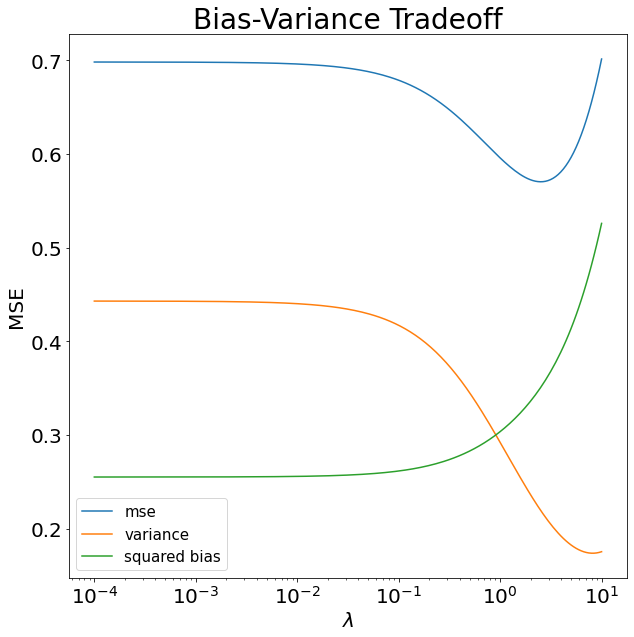
\includegraphics[scale=0.30]{Img/bias_var_tradeoff.png}%\hspace{-1.2cm}
        \centering
    \end{figure}
\end{frame}
%---------------------------------------------------------------------------%
\begin{frame}[fragile]
    \frametitle{DGP setup}
        $$
        y= X\beta + \varepsilon, \quad \text{with} \quad \varepsilon \sim \mathcal{N}_{n}(0, 1)
        $$

        $\textstyle X_{nxp} \sim \mathcal{N}(0, 1)$ such that the pairwise correlation between $x_{i}$ and $x_{j}$ is expressed as \\ 
        
        $$
        corr(\textit{i,j}) = \text{correlation factor} ^ \left|{i - j}\right|,
        $$\\ 
        
        where the correlation factor takes on a value between 0 and 1.
\end{frame}
%---------------------------------------------------------------------------%
\begin{frame}[fragile]
\frametitle{Minimum Test MSE (Case 1)}

\begin{block}{Set up}
    \begin{itemize}
        \item High dimensionality with varying sparsity, no multicollinearity. 
        \item $n = 30$
        \item $p = 35$
        \item All non-zero $\beta = 2$. 
    \end{itemize}
\end{block} \\

\begin{center}
    
    \begin{tabular}{||c c c c||} 
         \hline
          & High Sparsity & Med Sparsity & Low Sparsity \\ [0.5ex] 
          Model & (10 non-zero $\beta$'s) & (20 non-zero $\beta$'s) & (35 non-zero $\beta$'s) \\ [0.5ex]
         \hline\hline
         Ridge & 12.544 & 23.895 & \cellcolor{pink!60}36.074\\ 
         \hline
         Elnet (Naive), 0.2 & 10.182 & \cellcolor{pink!60}21.360 & 40.366 \\
         \hline
         Elnet (Naive), 0.5 & 8.760 & 21.687 & 46.961\\
        \hline
         Elnet (Naive), 0.7 & 7.421 & 22.380 & 52.046\\
        \hline
         Lasso & \cellcolor{pink!60}5.903 & 24.090 & 60.170\\
        \hline
    \end{tabular}

\end{center}
\end{frame}
%---------------------------------------------------------------------------%
\begin{frame}[fragile]
\frametitle{Minimum Test MSE (Case 2)}

\begin{block}{Set up}
    \begin{itemize}
        \item Low dimensionality with varying sparsity, moderate to high pairwise correlation (corr. factor = 0.8).  
        \item $n = 30$, $p = 10$
        \item All non-zero $\beta = 2$. 
    \end{itemize}
\end{block} \\

\begin{center}
    
    \begin{tabular}{||c c c c||} 
         \hline
          & High Sparsity & Med Sparsity & Low Sparsity \\ [0.5ex] 
          Model & (3 non-zero $\beta$'s) & (7 non-zero $\beta$'s) & (10 non-zero $\beta$'s) \\ [0.5ex]
         \hline\hline
         Ridge & 0.570 & 0.270 & \cellcolor{pink!60}1.140 \\ 
         \hline
         Elnet (Naive), 0.2 & 0.572 & 0.265 & 1.149 \\
         \hline
         Elnet (Naive), 0.5 & 0.577 & 0.246 & 1.164\\
        \hline
         Elnet (Naive), 0.7 & \cellcolor{pink!60}0.552 & \cellcolor{pink!60}0.218 & 1.166\\
        \hline
         Lasso & 0.607 & 0.298 & 1.166\\
        \hline
    \end{tabular}

\end{center}
\end{frame}
%---------------------------------------------------------------------------%
\begin{frame}[fragile]
\frametitle{Minimum Test MSE (Case 3)}

\begin{block}{Set up}
    \begin{itemize}
        \item Low dimensionality with high sparsity, varying degrees of pairwise correlation.  
        \item $n = 20$
        \item $p = 8$
        \item $\beta = (3, 1.5, 0, 0, 2, 0, 0, 0)$
    \end{itemize}
\end{block} \\

\begin{center}
    
    \begin{tabular}{||c c c c||} 
         \hline
          & Low Pairwise Corr. & Med Pairwise Corr. & High Pairwise Corr. \\ [0.5ex] 
          Model & (corr. factor = 0.1) & (corr. factor = 0.3) & (corr. factor = 0.7)\\ [0.5ex]
         \hline\hline
         Ridge & 1.238 & 2.071 & 0.905\\ 
         \hline
         Elnet (Naive), 0.2 & 1.160 & 2.034 & 0.889\\
         \hline
         Elnet (Naive), 0.5 & 0.979 & 1.897 & 0.864\\
        \hline
         Elnet (Naive), 0.7 & 0.828 & 1.724 & 0.851\\
        \hline
         Lasso & \cellcolor{pink!60}0.600 & \cellcolor{pink!60}1.340 & \cellcolor{pink!60}0.829\\
        \hline
    \end{tabular}

\end{center}
\end{frame}
%---------------------------------------------------------------------------%
\begin{frame}[fragile]
\frametitle{Minimum Test MSE (Case 4)}

\begin{block}{Set up}
    \begin{itemize}
        \item Low dimensionality with no sparsity, varying degrees of pairwise correlation.
        \item $n = 20$
        \item $p = 8$
        \item All $\beta = 0.85$
    \end{itemize}
\end{block} \\

\begin{center}
    
    \begin{tabular}{||c c c c||} 
         \hline
          & Low Pairwise Corr. & Med Pairwise Corr. & High Pairwise Corr. \\ [0.5ex] 
          Model & (corr. factor = 0.1) & (corr. factor = 0.3) & (corr. factor = 0.7)\\ [0.5ex]
         \hline\hline
         Ridge & \cellcolor{pink!60}2.471 & \cellcolor{pink!60}0.521 & \cellcolor{pink!60}0.736\\ 
         \hline
         Elnet (Naive), 0.2 & 2.506 & 0.585 & 0.772\\
         \hline
         Elnet (Naive), 0.5 & 2.542 & 0.882 & 0.831\\
        \hline
         Elnet (Naive), 0.7 & 2.548 & 1.124 & 0.867\\
        \hline
         Lasso & 2.548 & 1.532 & 0.906\\
        \hline
    \end{tabular}

\end{center}
\end{frame}
%---------------------------------------------------------------------------%
\begin{frame}[fragile]
\frametitle{Minimum Test MSE (Case 5)}

\begin{block}{Set up}
    \begin{itemize}
        \item High dimensionality with high sparsity, varying degrees of pairwise correlation.  
        \item $n = 30$
        \item $p = 35$
        \item 10 non-zero $\beta = 2$
    \end{itemize}
\end{block} \\

\begin{center}
    
    \begin{tabular}{||c c c c||} 
         \hline
          & Low Pairwise Corr. & Med Pairwise Corr. & High Pairwise Corr. \\ [0.5ex] 
          Model & (corr. factor = 0.1) & (corr. factor = 0.3) & (corr. factor = 0.7)\\ [0.5ex]
         \hline\hline
         Ridge & 9.412 & 15.714 & 3.263\\ 
         \hline
         Elnet (Naive), 0.2 & 7.932 & 11.092 & 2.659\\
         \hline
         Elnet (Naive), 0.5 & 6.049 & 10.505 & 1.882\\
        \hline
         Elnet (Naive), 0.7 & 5.122 & 8.570 & \cellcolor{pink!60}1.589 \\
        \hline
         Lasso & \cellcolor{pink!60}4.079 & \cellcolor{pink!60}6.575 & 1.716 \\
        \hline
    \end{tabular}

\end{center}
\end{frame}
%---------------------------------------------------------------------------%
\begin{frame}[fragile]
        \begin{figure}[b]
        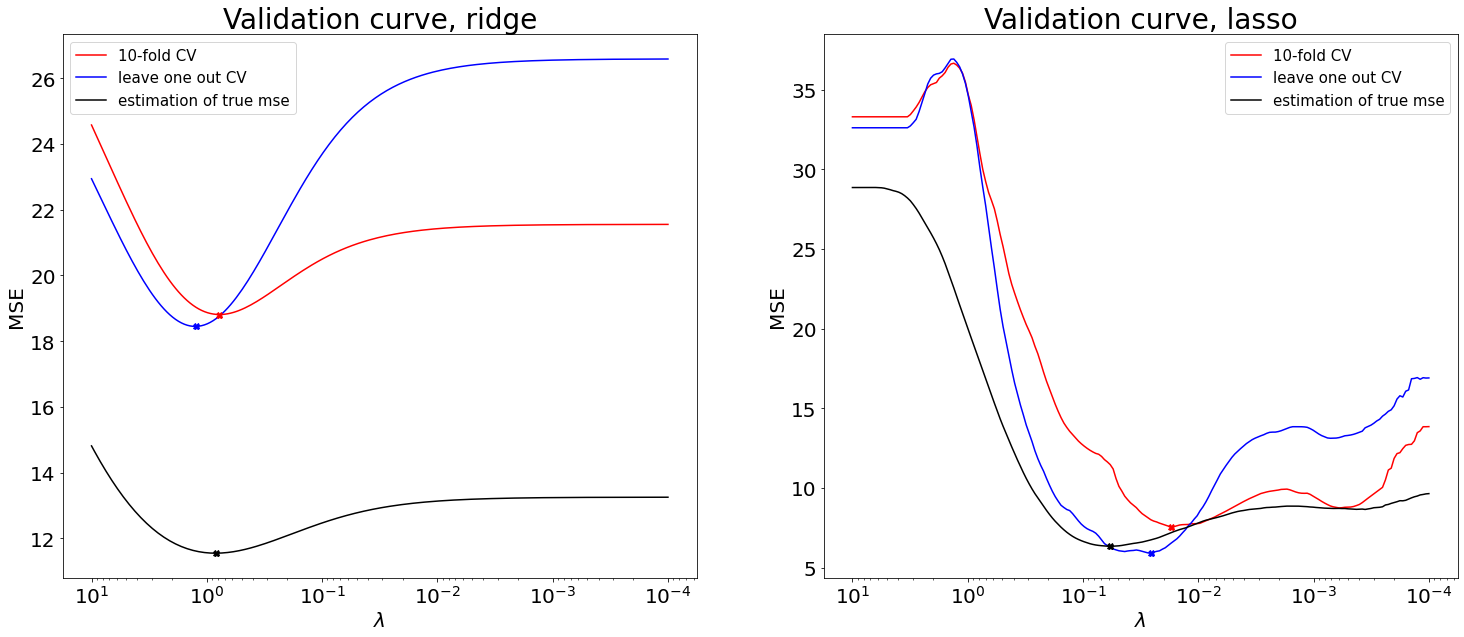
\includegraphics[scale=0.27]{Img/CV_simulation.png}%\hspace{-1.2cm}
        \centering
    \end{figure}
\end{frame}
%---------------------------------------------------------------------------%

%
%->> Data application
%---------------------------------------------------------------------------%
%---------------------------------------------------------------------------%
\lecture{Research Presentation}{lec_present_application}
%---------------------------------------------------------------------------%
\section{Data Application}%
%---------------------------------------------------------------------------%
\begin{frame}[fragile]
    \frametitle{Prostate Cancer Data Set}
    \begin{itemize}
        \item What is the relationship between log prostate specific antigen (lpsa) levels, which is elevated in men with prostate cancer, and other clinical measures $(p=8)$
        \item $n=97$
        \item For comparability we use the same train-test split as \cite{zou2005regularization}
        \item High correlation between
            \begin{itemize}
            \item lcp \textit{(log of capsular penetration)} and lcavol \textit{(log cancer volume)}
            \item svi \textit{(seminal vesicle invasion)} and lcp
            \item pgg45 \textit{(percent of Gleason score 4 or 5)} and gleason \textit{(Gleason score)}
            \item pgg45 and lcp
            \end{itemize}
    \end{itemize}
\end{frame}
%---------------------------------------------------------------------------%
\begin{frame}
\frametitle{Correlation Matrix}
    \begin{figure}
    %\column{.5\textwidth}
        \centering
        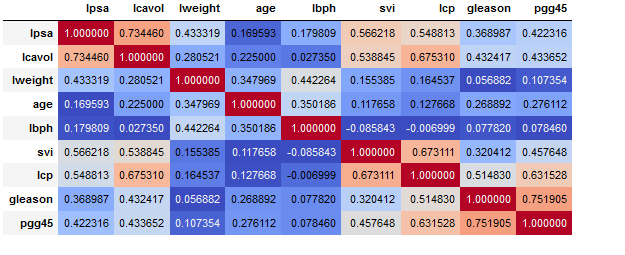
\includegraphics[width=11cm,height=5.5cm, left]{Img/corr_table.png}
    \end{figure}
\end{frame}
%---------------------------------------------------------------------------%
\begin{frame}
%\begin{columns}[t]
%\column{.5\textwidth}
\centering
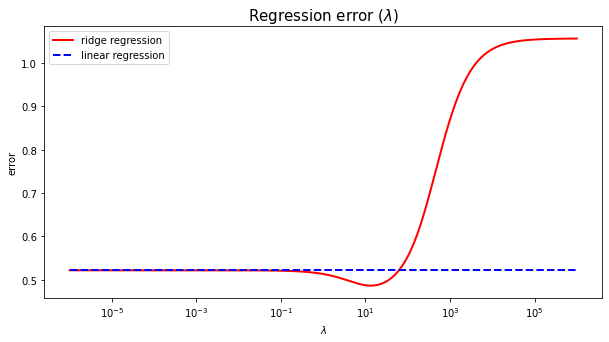
\includegraphics[width=7cm,height=4cm, left]{Img/data_ridge_vs_lambda.png}
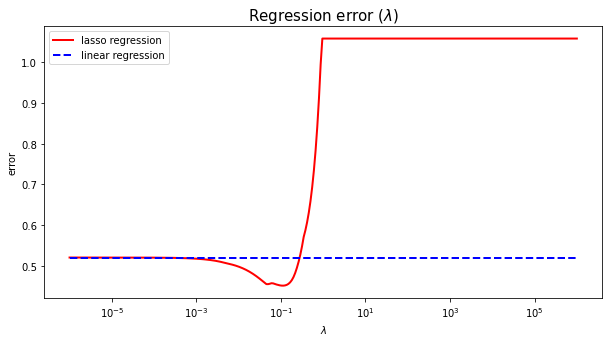
\includegraphics[width=7cm,height=4cm, right]{Img/data_lasso_vs_lambda.png}\\
%\column{1.0\textwidth}
\centering
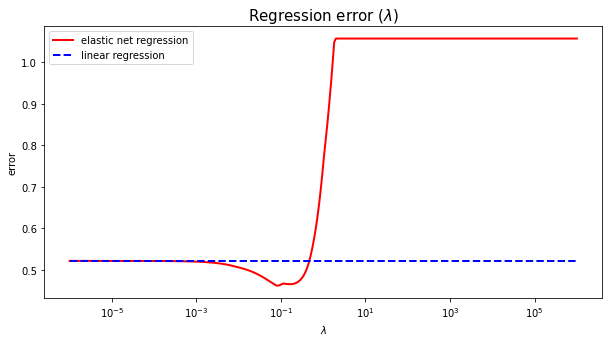
\includegraphics[width=7cm,height=4cm, center]{Img/data_elnet_vs_lambda.png}\\
%\end{columns}
\end{frame}


%---------------------------------------------------------------------------%
\begin{frame}
%\begin{columns}[t]
%\column{.5\textwidth}
\centering
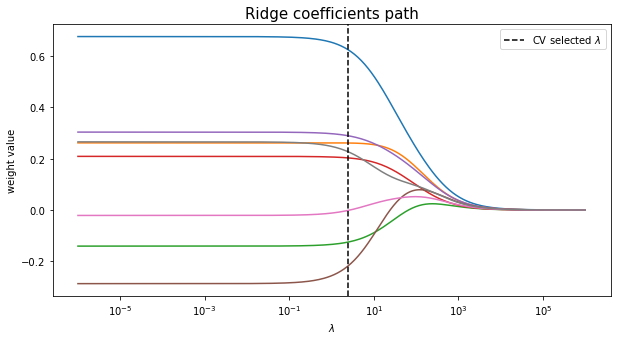
\includegraphics[width=7cm,height=4cm, left]{Img/data_ridge_coef_path.png}
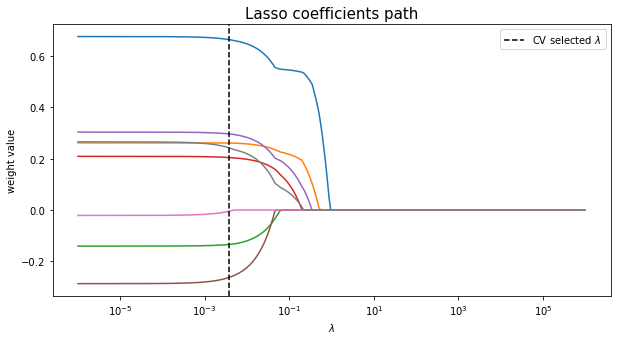
\includegraphics[width=7cm,height=4cm, right]{Img/data_lasso_coef_path.png}\\
%\column{1.0\textwidth}
\centering
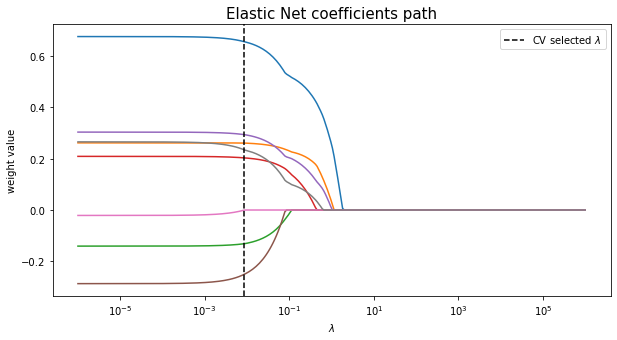
\includegraphics[width=7cm,height=4cm, center]{Img/data_elnet_coef_path.png}\\
%\end{columns}
\end{frame}

%---------------------------------------------------------------------------%
\begin{frame}
\frametitle{Model Selection}
\begin{center}
\small
\begin{tabular}{||c c c c||} 
 \hline
 Model & Test MSE (with 10-fold CV) & Test MSE (AIC) & Variable Selection\\ [0.5ex] 
 \hline\hline
 Linear & 0.5213 & - & All\\ 
 \hline
 Ridge & 0.5043 & - & All\\
 \hline
 Lasso & 0.5112 & - & All\\
 \hline
 Elastic Net (Naive) & 0.5043 & - & All\\
 \hline
 LARS & 0.5084 & 0.5033 & lcavol, lweight, lbph, \\ & & & svi, pgg45\\
 \hline
\end{tabular}
\end{center}\\

\begin{block}{Takeaway}
\begin{itemize}
\item Naive elastic net performs as well as ridge, also reported by \cite{zou2005regularization}
\item Lasso performs best if LARS algorithm is implemented and AIC is used for tuning $\lambda$. It performs variable selection as in \cite{zou2005regularization}.
\end{itemize}
\end{block}

\end{frame}%
%---------------------------------------------------------------------------%
%->> Conclusion
%---------------------------------------------------------------------------%
%---------------------------------------------------------------------------%
\lecture{Research Presentation}{lec_present_conclude}
%---------------------------------------------------------------------------%
\section{Conclusion}
%------------------------------------------------------------


\begin{frame}
    \begin{figure}
    %\column{.5\textwidth}
        \centering
        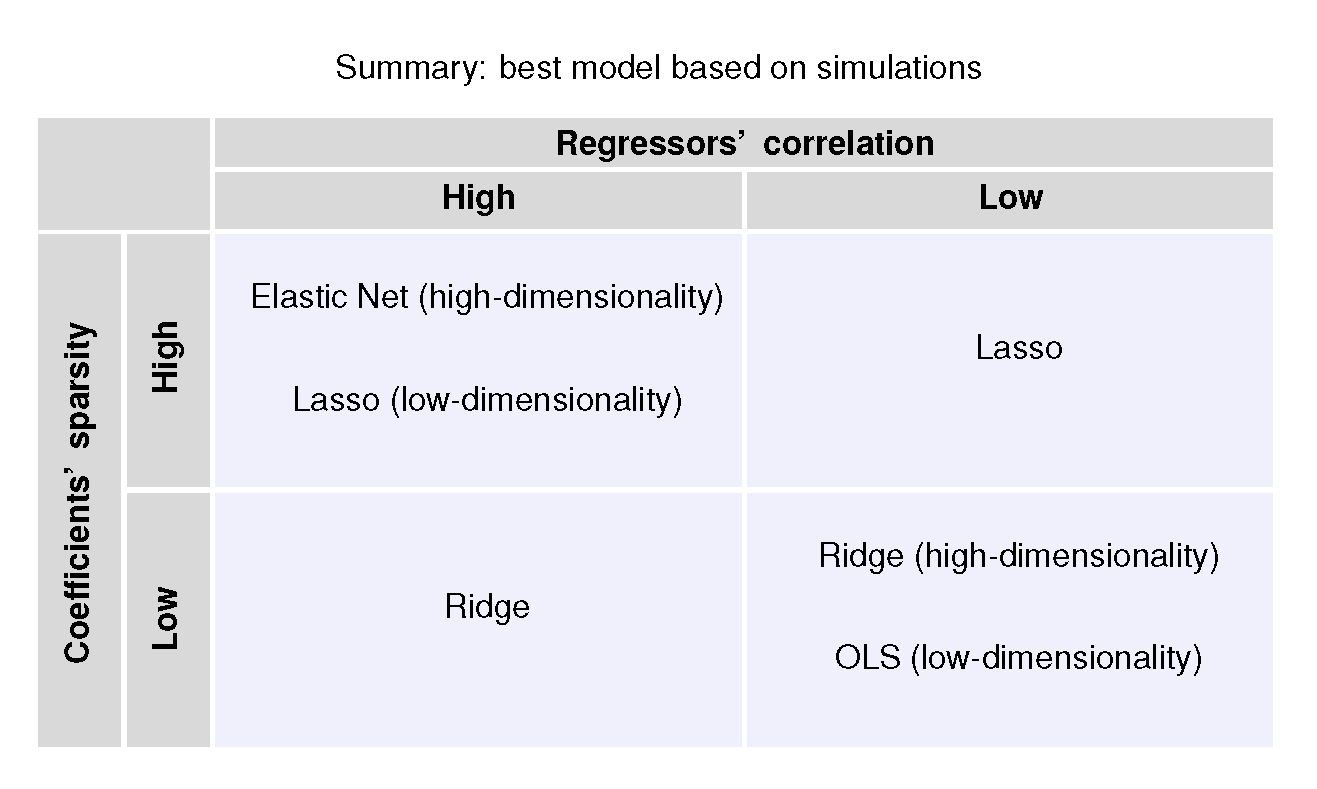
\includegraphics[width=11cm,height=5.5cm, left]{Img/2x2table.png}
    \end{figure}
    
\begin{itemize}
        \item The data application is in line with \textit{Case 2} of our simulation study.
    \end{itemize}
\end{frame}
%%---------------------------------------------------------------------------%%
%---------------------------------------------------------------------------%
%
%-
%-> Backmatter
%-
%---------------------------------------------------------------------------%
%->> Backmatter
%---------------------------------------------------------------------------%
%->> Question
%---------------------------------------------------------------------------%
\lecture{Research Presentation}{lec_present_question}
%---------------------------------------------------------------------------%
{%
\begin{frame}[plain]
    \begin{center}
        {\large\bfseries {Thank you for your attention!}}
    \end{center}
    \tikzart[t=p,x=0,y=-4,w=4]{bonn-logo}
    \addtocounter{framenumber}{-1}% modify the counter to exclude a frame from total count
\end{frame}
}
%---------------------------------------------------------------------------%
%->> Appendix
%---------------------------------------------------------------------------%
\lecture{Research Presentation}{lec_present_appendix}
%---------------------------------------------------------------------------%
%\appendix% begin appendix
%\newcounter{finalframe}% define a new counter
%\setcounter{finalframe}{\value{framenumber}}% save regular slides counter
%---------------------------------------------------------------------------%
%\section{\appendixname}% the end page.
%\frame{\tableofcontents}% outline for appendix
%---------------------------------------------------------------------------%
%\subsection{Classic Beamer Style}
%---------------------------------------------------------------------------%
\begin{frame}[fragile]
\frametitle{Appendix}
    \begin{figure}[b]
        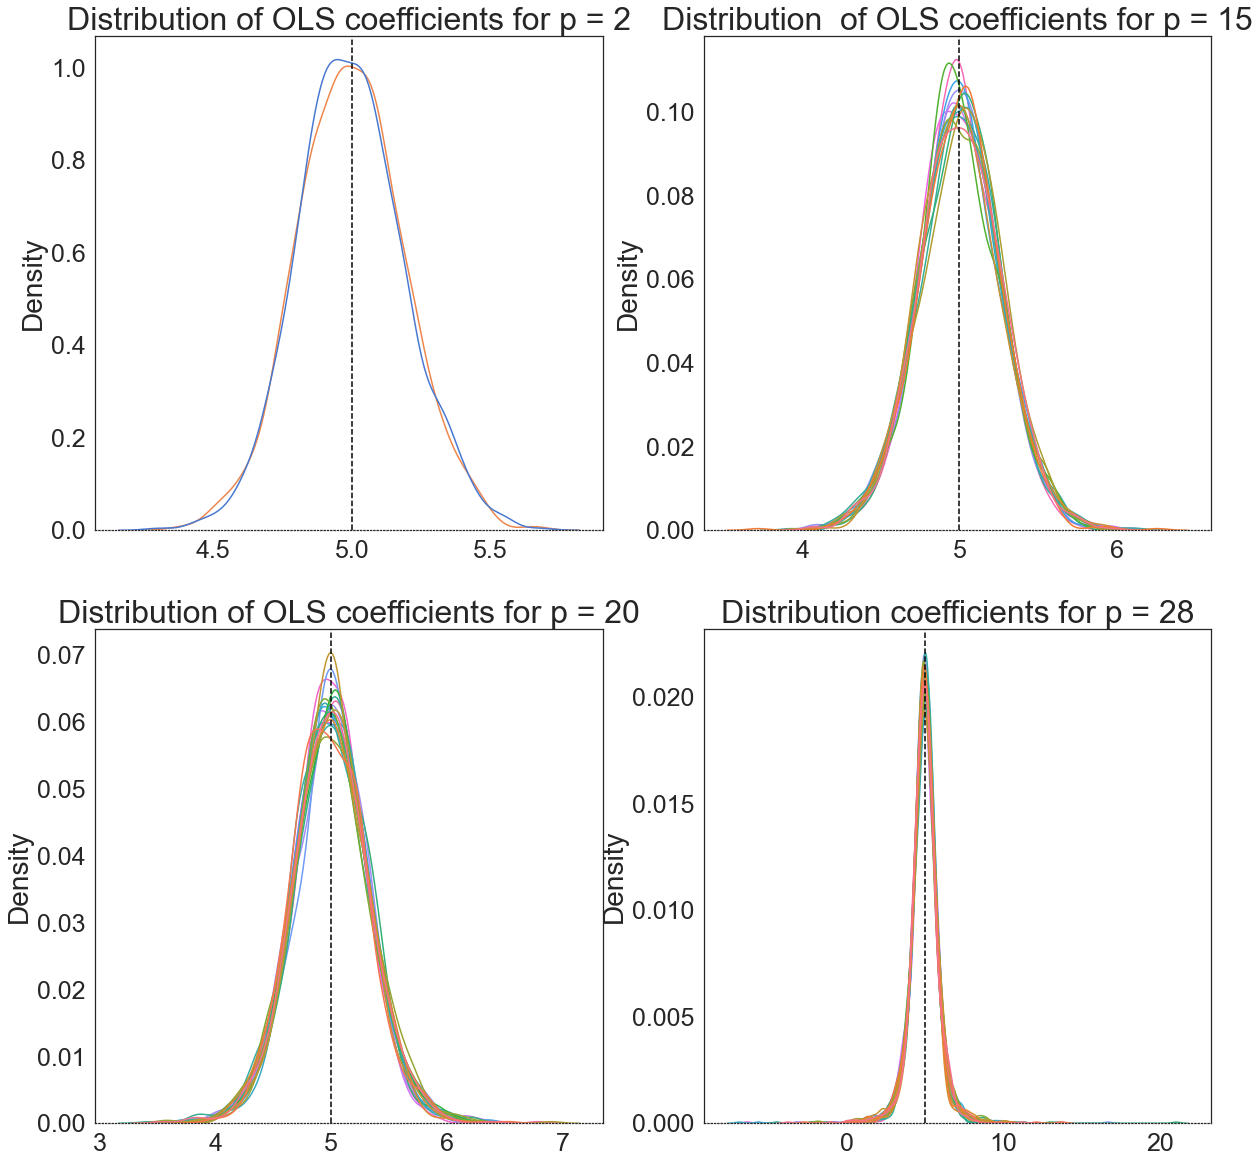
\includegraphics[scale=0.17]{Img/ols_distr.png}
        \centering
    \end{figure}
\end{frame}
%---------------------------------------------------------------------------%
\begin{frame}[fragile]
    \frametitle{Appendix}
    \begin{figure}[c]
        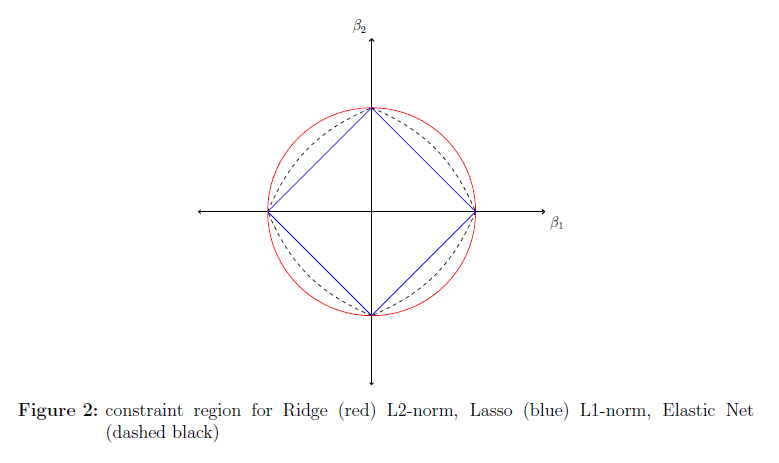
\includegraphics[scale=0.57]{Img/constraints.png}\hspace{-1.2cm}
        \centering
    \end{figure}
\end{frame}
%---------------------------------------------------------------------------%
\begin{frame}[fragile]
    \frametitle{Appendix}
    \begin{figure}[b]
        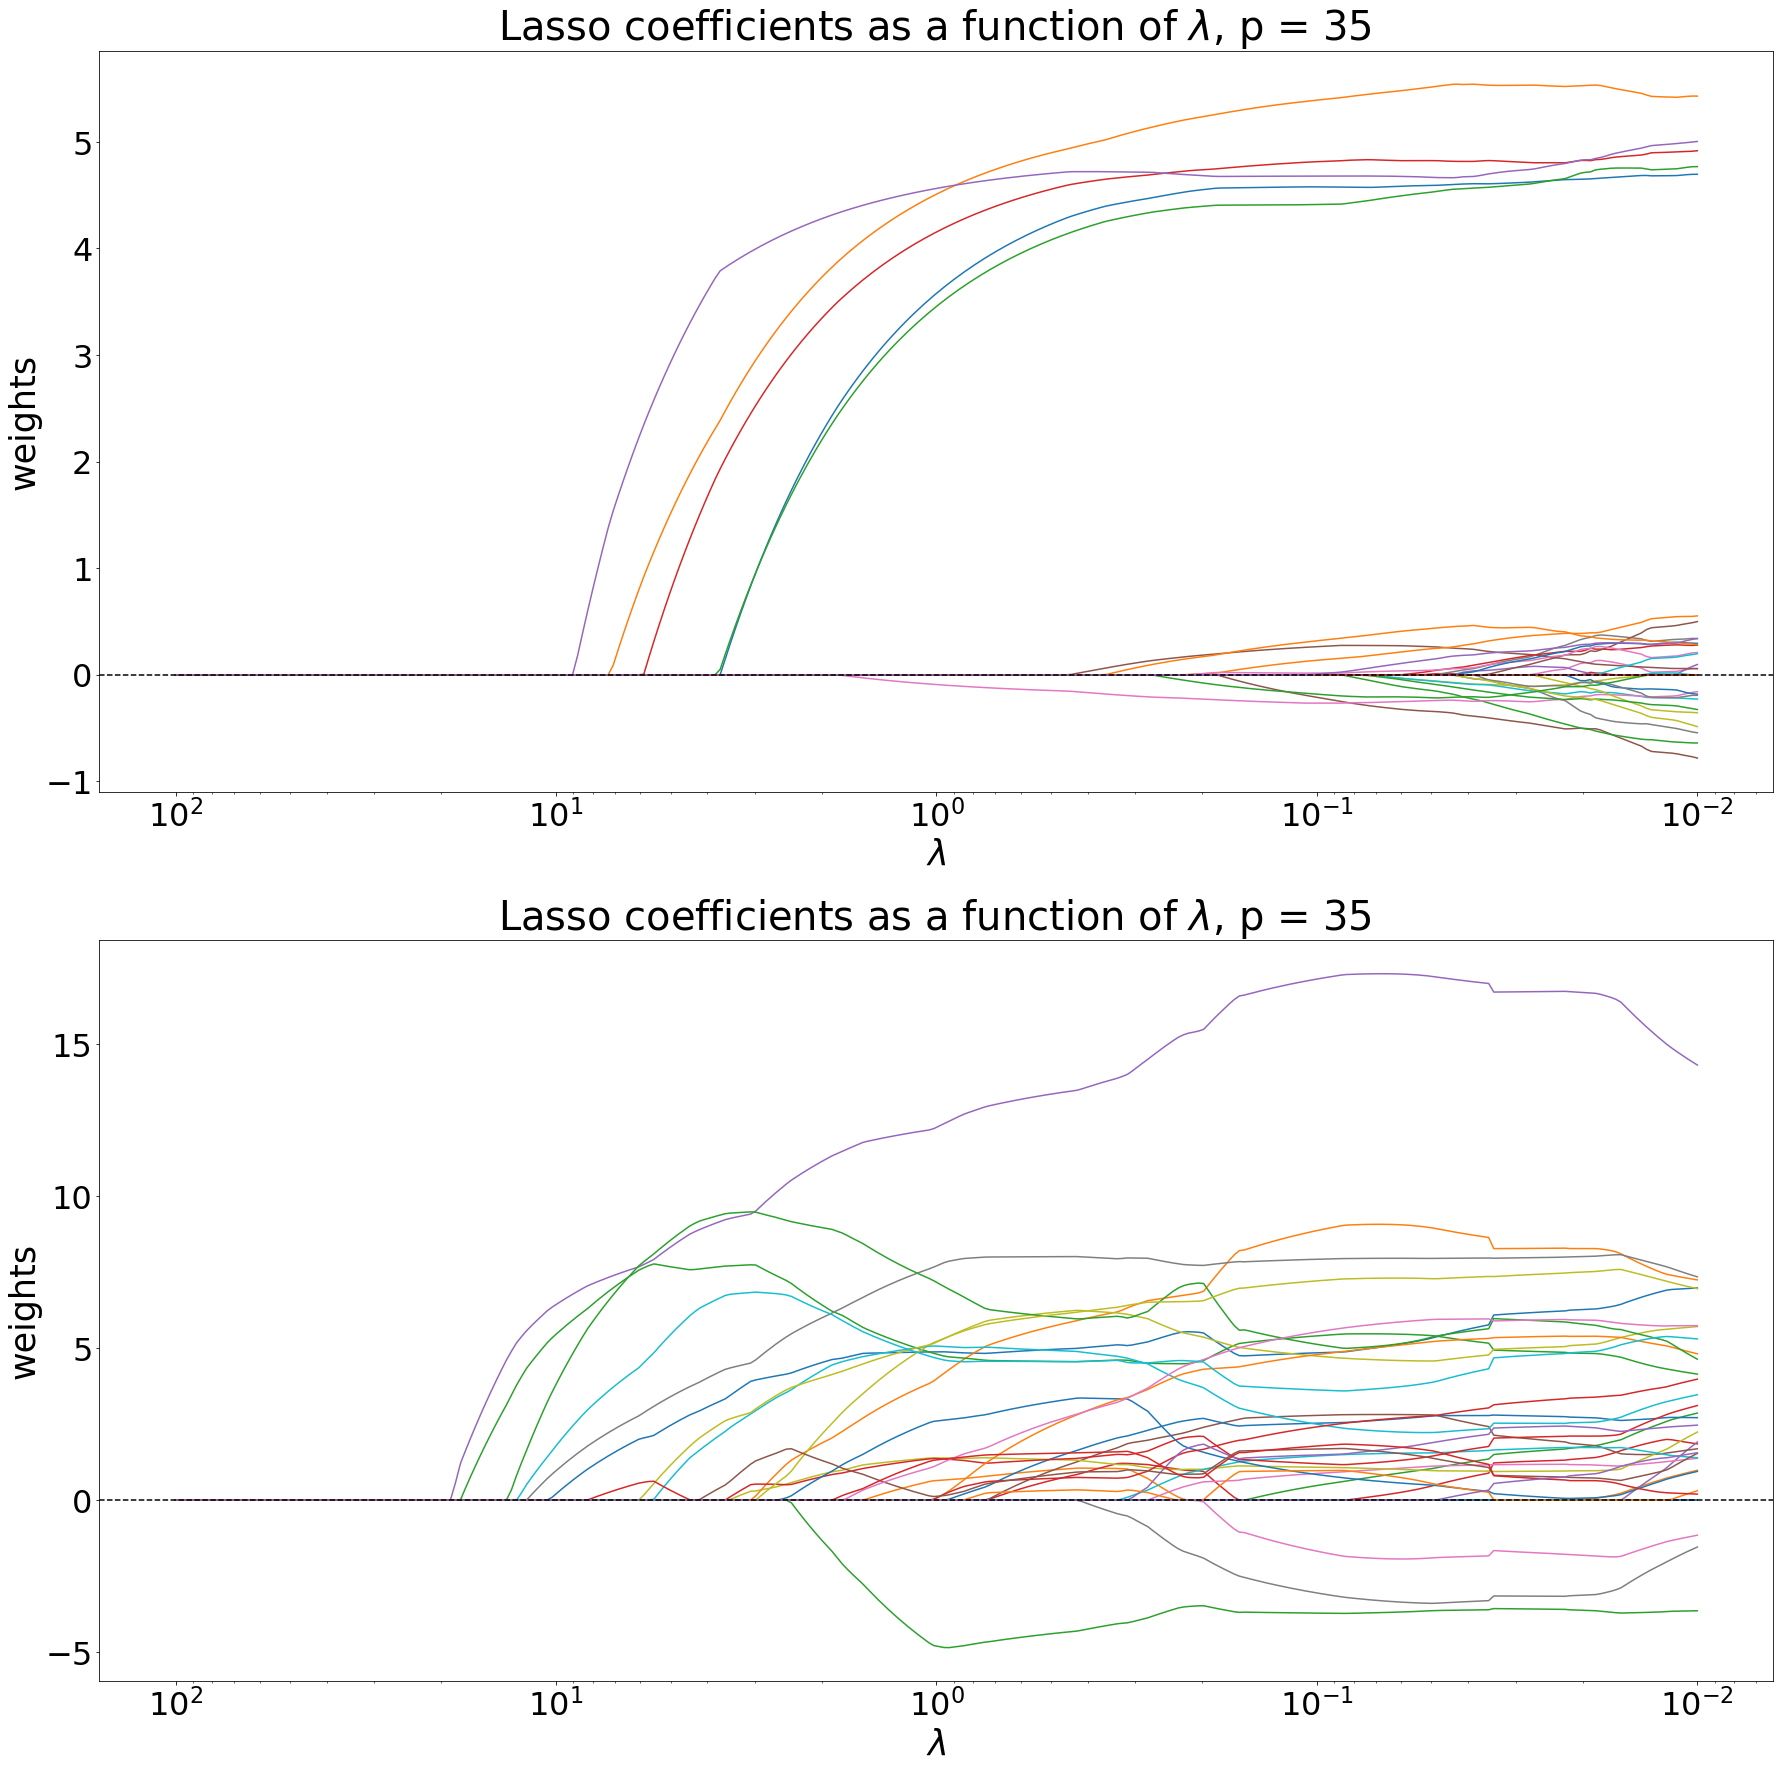
\includegraphics[scale=0.13]{Img/lasso_plot_betas.png}
        \centering
    \end{figure}
\end{frame}
%---------------------------------------------------------------------------%
\begin{frame}[fragile]
    \frametitle{Appendix}
    \begin{itemize}
        \item We used a \textit{10-fold cross validation} approach to find the optimal value of the tuning parameter.
    \end{itemize}
    \begin{align}
    \label{}
    CV_{(k)}=\frac{1}{k}\sum_{i=1}^{k} \: MSE_i
    \end{align}
    \begin{itemize}
        \item We identify the model with the lowest test error.
        \item We identify the $\lambda$ value that minimizes the MSE and then plug it back into the model of interest.
    \end{itemize}
\end{frame}
%---------------------------------------------------------------------------%
\begin{frame}[fragile]
    \frametitle{Appendix}
    \textbf{Least-angle regression (LARS) (\cite{efron2003lars})} \\
    \begin{itemize}
        \item Provides an extremely efficient algorithm for computing the entire lasso path.
        \item Lasso is a variant of the LARS procedure.
        \item LARS algorithm:
        \begin{enumerate}
            \item Standardize predictors.
            \item Find predictor $x_j$ that is most correlated with $y$.
            \item Move $\beta_j$ from 0 towards least-squares coefficient until  $x_k$ has as much correlation with the current residual as does $x_j$.
            \item Move $\beta_j$ and $\beta_k$ in the direction of the joint least squares coefficient of the current residual on ($x_j$, $x_k$), until $x_l$ has as much correlation with the current residual.
            \item Continue until all $p$ have been entered.
            \item \textit{If a non-zero coefficient hits zero, drop the corresponding variable from the active set of variables and recompute the current joint least squares direction.}
        \end{enumerate}
    \end{itemize}
\end{frame}
%---------------------------------------------------------------------------%
\lecture{Research Presentation}{lec_present_ref}
%---------------------------------------------------------------------------%
\subsection{References}
%---------------------------------------------------------------------------%
\begin{frame}[allowframebreaks]
    \frametitle{References}
    \nocite{*}
    \printbibliography[heading=none]%
\end{frame}
%---------------------------------------------------------------------------%
%\setcounter{framenumber}{\value{finalframe}}% rectify the slides counter
%---------------------------------------------------------------------------%
%
\end{document}
%---------------------------------------------------------------------------%
